%%%%%%%%%%%%%%%%%%%%%%%%%%%%%%%%%%%%%%%%%%%%%%%%%%%%%%%%%%%%%%%%%%%%%%%%%%%%%%%%%%%%%%
% Copyright © 2023 Haochen WANG (王昊辰).
% Contact: whch.o@outlook.com: +86 18921173379; +31 0633217019; +44 07579859390
%YinRen-YuShu 3401, WuXi, JiangSu, PRC; 214011 (中华人民共和国,江苏,无锡,银仁-御墅,3401; 214011)
%
% This LaTeX template has been developed and produced by Haochen WANG (王昊辰).
% Excluding the written content, this template is distributed under a Creative Commons Attribution-NonCommercial 4.0 International License (CC BY-NC 4.0).
% Please adhere to the terms of this license when utilising this template.
% Comprehensive information about the license can be found at:
%https://creativecommons.org/licenses/by-nc/4.0/
%%%%%%%%%%%%%%%%%%%%%%%%%%%%%%%%%%%%%%%%%%%%%%%%%%%%%%%%%%%%%%%%%%%%%%%%%%%%%%%%%%%%%%
\documentclass{book}
\usepackage[twoside=true,inner=19mm,outer=12.7mm,top=20mm,bottom=20mm,paperwidth=6in,paperheight=9in]{geometry} %页边距
\usepackage{emptypage} 
\usepackage[UTF8]{ctex} % 支持中文
\usepackage{fontspec} % 使用fontspec宏包
%\setmainfont{CMU Serif} % 设置英文字体CMU
\setmainfont{Liberation Serif} % 自由衬线
\setCJKmainfont{SourceHanSerifSC-Medium.otf} % 设置中文正文字体为思源宋体,一般粗
\newCJKfontfamily\sectionfont{SourceHanSerifSC-Heavy.otf} % 设置中文标题字体为思源宋体,粗

%设置目录自号
\usepackage{tocloft}
\renewcommand{\cftsecfont}{\fontsize{10.5pt}{17pt}\selectfont}  % 设定 section 标题的字号
\renewcommand{\cftsubsecfont}{\fontsize{10.5pt}{17pt}\selectfont} % 设定 subsection 标题的字号
\renewcommand{\cftsubsubsecfont}{\fontsize{10.5pt}{17pt}\selectfont} % 设定 subsection 标题的字号
\renewcommand{\cftparafont}{\fontsize{10.5pt}{17pt}\selectfont}  % 设定 paragraph 标题的字号
\renewcommand{\cftsubparafont}{\fontsize{10.5pt}{17pt}\selectfont} % 设定 subparagraph 标题的字号

\usepackage{lipsum} % 用于生成随机文字
\usepackage{ccicons} % 创作共享图标
\usepackage{hyperref} % 提供超链接功能
\hypersetup{
    colorlinks=false, %取消超链接的颜色
    pdfborder={0 0 1}, %显示超链接的下划线
    urlbordercolor={0 0 1} %设定超链接方框颜色
}
\usepackage{fancyhdr} % 添加fancyhdr宏包
\usepackage[ddmmyyyy]{datetime}%日期
\usepackage{indentfirst} % 用于段首缩进
\usepackage{ragged2e} % 用于对齐
\usepackage{tabularx} % 用于表格
\usepackage{indentfirst} % 添加indentfirst宏包,使所有的段落都在开始时自动缩进
\usepackage{titlesec} %用于设置标题
\usepackage{ulem} %下划线
\usepackage{pgfplots}%用于蜘蛛图
\pgfplotsset{compat=1.15} %用于蜘蛛图
\usepgfplotslibrary{polar}%用于蜘蛛图
\usepackage{wrapfig}%用于蜘蛛图
\usepackage{pdfpages}%pdf page
\usepackage{xcolor}%字体颜色
\definecolor{light-gray}{gray}{0.8}%定义颜色light-gray
\definecolor{dark-gray}{gray}{0.5}%定义颜色dark-gray
\usepackage{zhnumber} % 导入将数字转换为中文数字的宏包
%\renewcommand\thesection{\zhdigits*{\arabic{section}}} 
% 重定义section编号的显示方式,将阿拉伯数字转换为中文的大写数字,“壹、贰、叁”形式。
\setcounter{secnumdepth}{5} % 使得五级标题都有编号
\setcounter{tocdepth}{5} % 使得五级标题都能在目录中显示
\usepackage{pgfgantt} %gantt chart

%设置chapter样式
\titleformat{\chapter}[block] % "block"样式以匹配其他标题样式
{\normalfont\fontsize{35}{30}\bfseries\sectionfont} %标题字号,字体
{} %去掉编号
{0pt} %标题和标题名之间的空格
{\thispagestyle{fancy}} % 在每个章节的开始使用 fancy 页脚样式
\setcounter{chapter}{-1}%目录从0开始算

%\titlespacing*{\chapter}{0pt}{0pt}{20pt} %调整空白空间


%设置section样式
\titleformat{\section}
{\normalfont\fontsize{14}{27}\bfseries\sectionfont} %子标题字号,字体
{\thesection}
{1em}
{}

%设置subsection样式
\titleformat{\subsection}
{\normalfont\fontsize{11}{25}\bfseries\sectionfont} %子标题字号,字体
{\thesubsection}
{1em}
{}

%设置subsubsection样式
\titleformat{\subsubsection}
{\normalfont\fontsize{10.5}{25}\bfseries\sectionfont} %子标题字号,字体
{\thesubsubsection}
{1em}
{}

\pagestyle{fancy} % 设置页面样式为fancy
\fancyhead{} % 清空页眉设置
\fancyfoot{} % 清空页脚设置
\fancyhead[LE,RO]{\textbf{\fontsize{10.5}{17}\sectionfont\textcolor{dark-gray}\rightmark}} %右上角打上subsection
\renewcommand{\headrulewidth}{0pt} % 去除页眉横线
\fancyfoot[LE,RO]{\fontsize{11}{17}\textbf{\thepage}} %页码
\fancyfoot[RE,LO]{\textcolor{light-gray}{Copyright © 2023 by Haochen WANG (王昊辰)}}

\setlength\parindent{2em} %首行缩进

\newlength{\betsubsec}
\setlength{\betsubsec}{0.01\textheight}  % 定义subsection间的空白




% 修改目录
\renewcommand{\contentsname}{\fontsize{35}{30}\bfseries\sectionfont{目录}} 

\newenvironment{toc}{
  \pagestyle{empty} % 在环境开始时设置页面样式为空
  \tableofcontents
  \clearpage
}{%
  \pagestyle{fancy} % 在环境结束时重新设置页面样式
}

\cftsetindents{chapter}{0em}{1em} %改缩进
\cftsetindents{section}{1em}{2em}
\cftsetindents{subsection}{2em}{2.8em}
\cftsetindents{subsubsection}{3em}{3.1em}
\cftsetindents{paragraph}{4em}{3.4em}

%改enurmate样式
\usepackage{enumitem} % 导入enumitem宏包
\setlist[enumerate]{itemsep=0pt} % 设置所有的enumerate环境中项目之间的间距

%正式开始文档
%%%%%%%%%%%%%%%%%%%%%%%%%%%%%%%%%%%%%%%

\begin{document}

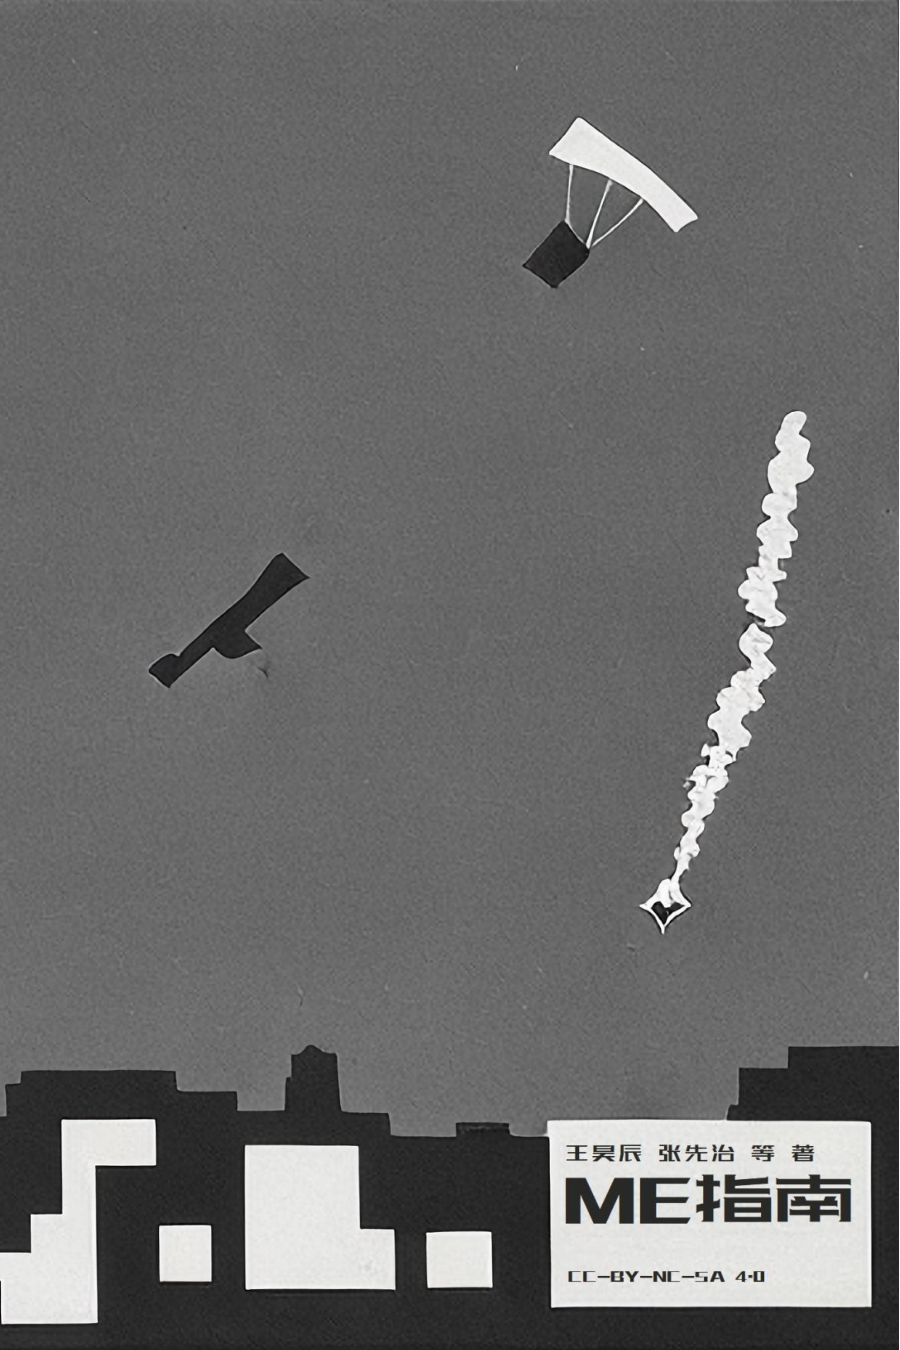
\includepdf[pages=1,fitpaper=true]{cover.pdf} %封面

\begin{titlepage} % 开始创建扉页
\newgeometry{vmargin={20mm}, hmargin={19mm,12.7mm}}  % 设置自定义边距

\vspace*{\stretch{0.382}} % 使用黄金分割比例来分配空间

% 标题部分
\begin{flushright} % 使用 flushright 环境来实现右对齐
\fontsize{40}{10}\bfseries\sectionfont{ME指南} % \fontsize 设置特大号字体,\textbf 使文字加粗
\end{flushright}

\vspace*{\stretch{0.236}} % 使用黄金分割比例来分配空间

% 作者部分
\begin{flushright} % 使用 flushright 环境来实现右对齐
\fontsize{24}{0}\selectfont{王昊辰\textsuperscript{1}} % \fontsize 设置较大号字体,\textbf 使文字加粗
\end{flushright}

\vspace*{\stretch{0.05}} % 使用黄金分割比例来分配空间

% co-author部分
\begin{flushright} % 使用 flushright 环境来实现右对齐
\fontsize{16}{0}\selectfont{张先治\textsuperscript{2}、马润禹\textsuperscript{3}、刘彦菁\textsuperscript{4}、祁晨晨\textsuperscript{5}、孙天辰\textsuperscript{6} 等} % Co-author写上
\end{flushright}

\vspace*{\stretch{0.382}} % 使用黄金分割比例来分配空间

% 版权信息部分
\begin{flushright} 
\fontsize{7}{8}\selectfont\textcolor{dark-gray}{
{Address: YinRen-YuShu 3401, WuXi, JiangSu, P.R.C.; 214011}\\
{Contact: \href{mailto:whch.o@outlook.com}{whch.o@outlook.com}}\\
{Unless otherwise noted, contents within this brochure are licensed under the \ccbyncsa\ \href{http://creativecommons.org/licenses/by-nc-sa/4.0/}{\uline{CC BY-NC-SA 4.0}.}}\\
{Updated as of \today}}
\end{flushright}

\vspace*{\stretch{0.618}} % 使用黄金分割比例来分配空间

\end{titlepage} % 结束创建标题页

\cleardoublepage
% 在生成目录前将页面样式设置为空
\pagestyle{empty}
\addtocontents{toc}{\protect\thispagestyle{empty}} % 在这里插入
\begin{toc} % 使用自定义环境生成目录
\end{toc}
% 设置此页样式为空

\thispagestyle{fancy} % Reset the style immediately after the table of contents
\pagestyle{fancy} % 在新的一章开始时再将页面样式重新设置为fancy
%\pagenumbering{arabic} % 重新开始页码计数,并应用页眉页脚样式
\addtocounter{page}{-6}
\fontsize{10.5}{16}\selectfont % 字体大小和行距

\cleardoublepage
\newpage\chapter{ 序}
\section{我的呓语}
已经一年了,很多时候,我都还在疑惑自己当时何以来到TUD,我那时候以为自己想要解开谜团,探索未知;幻想自己以汲取知识为裨益.我以为当时所在的英国本科满是混沌,我把希望与憧憬寄托在了这里,幻想里的乌有乡;和多少年前踏进小学,走入初中,到达高中,又闯入大学的一轮轮没有多少分别。和那时候又相似的,是总算抵达,却发觉究竟围城。

回头看看,是真的不知道自己决定背后的所以然。我似乎总是在自动驾驶;顺水而行,掺杂悲观的决策里面,度过了至今天大部分的岁月:那拉普拉斯的妖怪,一切的运动规律,过去将来,我虚无缥缈的主观能动,真的在宇宙大爆炸的一瞬间已经注定?《繁花》里面,小毛临死前讲,“上帝不响,像一切全由我定。”上帝不响,命运喧嚣;方舟里面,多少人竖起来石像;一轮又一轮的暮霭,岁月风化,层层叠叠。最后总归全部黑夜漫游,各奔归途。

但作为个人,我还是出发,还是启航。我继续满怀希望,依旧葬身大海。别人跟我讲,南岛民族其实是百越后裔;多少个千年过掉了,轮回又轮回,我的血脉,似乎和他们到底没多少不同。

总是觉得应该写个序,键盘敲敲,这些句子,垂头丧气。留学出发的行前,记忆里激情澎湃,无限憧憬,又几多焦虑;“This time tomorrow, where will we be ?” 那时候的我这样想着。如今的我回头望望,一天一天,过去的未来,浑芒光晕拨开,其实还是周而复始。地势坤,前路多少漫漫:这此刻行前的兴奋,清单里的未完成,辗转反侧的忧虑恐惧或其它;终归会在autopilot的飞驰里面;和自己无数已然经历的过去一样,巨大动量下,顺其自然间,不知不觉一溜烟,全部轰隆完成又远去离开。

有点感冒,又恰了点小酒,边写边默念着,嗓子都又有点哑掉了。星斗吱呀,杯酒涣散。有的时候自己真的都泄气了: 这世道普遍失落,其间眉头我终归解不开的,也懒得假装关心了。但又总自以为是,觉得力所能及的很多方面,多少能给点指引,帮忙散开些噪声氤氲的未知。

于是就有了这指南。尽管,我清晰地明白,无论如何,到底生来的宿命就是一而再的跌落又被吹散;陨石或者柳絮。西欧平原,风车旋转的确依旧;秋风日暮,时而为飞蛾,时而又幽暗烛火。蚍蜉撼树,我所想的,只是让这沧海一粟的我们,坠落得慢点再慢点。
\begin{flushright}
王昊辰;27/05/2023 于Delft
\end{flushright}

\vspace{\betsubsec} %section间留白
\section{一些说明}
这支指南;虽说以BMD命名;但或许于其它许多专业也应该是比较适用的。如封皮所言,所有内容,若非特地说明,则全部在\ccbyncsa\ \href{http://creativecommons.org/licenses/by-nc-sa/4.0/}{\uline{CC BY-NC-SA 4.0}}的License下。于遵守license要求的情境里,还请随意按照自己意愿需求更改使用。笔者乐于看到此作的衍生;希望它能够帮助更多的人;幻想它在长久未来里,一年又一年地不断丰富更新,于是流芳;帮笔者在赛博世界里面留下点今生今世的证据。

指南里的内容,上下辑两部分:其中上辑有关选课,也有关于第一年以外的实习与毕设;下辑则更多是生活方面:办银行卡,去医院,超市优惠之类。小册子里,所有以全英文标题命名的环节意味着其关乎课内;而若掺杂中文,则就更多偏向生活了。

课内部分的目录顺序,由于笔者本人的Track 是Biomechanical Design (BMD),故依照BMD课程的Form2内容及顺序进行了目录编排;BMD Form2 以外的课程,就一股脑地塞进了Alternative Electives的类别里面。虽说主要基于BMD,但鉴于Mechanical Engineering(ME),及Biomedical Engineering(BME)的可选课程有着诸多共通,因此或多或少的,对于整个ME及BME而言,都应有些参考价值吧;只是于BMD以外的读者,就可能需要在上辑的目录中自行搜索课程信息了。

小册子里,但凡挂着下划线的文字,全部都是可以点击的超链接;往往指引至上文或下文提及的相关地方。

本指南的pdf文件可以于如下链接获取:
\begin{enumerate}
\item \href{https://book.baige.me/view/c1l}{\uline{样本云(无需梯子,可在线阅读,最为推荐)}}
\item \href{https://wwkg.lanzoup.com/b04q5cmch}{\uline{蓝奏云(无需梯子,但时常不稳定),密码:TUD}}
\item \href{https://drive.google.com/drive/folders/1rxghlV072abqS7_6GpjdmStmXHPLw4bG?usp=sharing}{\uline{Google Drive}} 
\end{enumerate}

而构建此小册子的Latex代码全部都可于如下链接查看或使用:
\begin{enumerate}
\item \href{https://github.com/HochanWang/BMD-ZhiNan}{\uline{Github}}
\item \href{https://www.overleaf.com/9181971742xyhrjrdxdzkt}{\uline{Overleaf(随着了笔者的毕业,可能失效)}}
\end{enumerate}

当然,纸质版也可通过\href{https://www.lulu.com/shop/haochen-wang/me%E6%8C%87%E5%8D%97/paperback/product-8vmyjk.html?q=TUD&page=1&pageSize=4}{\uline{lulu.com 进行购买}},定价为网站最低要求的8欧元,除开印刷成本和抽成,笔者每本收入3.22欧元。全部收入,每当超过10欧元,笔者会全数捐给\href{https://chinaconcern.org/zh_hans/?fbclid=IwAR263C_R6_XiYRZrUrad-3TvXTMNcJAJWlTMwOiNIhiyCmAGR3GjPwBWH0w}{\uline{国际关心中国慈善协会(International China Concern)}},这是一家财务公开的,主要帮助中国大陆地区因为残疾,贫穷或仅仅因为性别原因就被遗弃儿童的慈善组织。其在荷兰地区的办事处受到荷兰监管机构的认可。

购买实体书籍后,如若有自己的捐赠偏好的话,也可以发送邮件或添加笔者社交媒体账号说明情况。

而要是有其它私人问题需要联系的话,也还请发邮件或添加笔者的社交媒体账号。笔者是2022年秋季入学Delft的;如果有幸这份文档传承许久,多年以后或许我关于Delft的印象会模糊过时,不确定是否还会受用。但笔者如果还在人世,不出意外总归还是尽量回答的,联系方式如下:
\begin{enumerate}
\item 邮箱:\href{mailto:whch.o@outlook.com}{whch.o@outlook.com}
\item 微信: b190552589
\item QQ: 506007201
\end{enumerate}

\begin{flushright}
王昊辰;17/06/2023
\end{flushright}


\cleardoublepage
\newpage\chapter[上辑:以Form2为纲]{上辑:\\以Form2为纲}
BMD的第一年,理想状态下需要依照Form2的要求,修满60学分的课程;但54学分修满,则已经可以开始第二年的Graduation Project。而若仅为保留在tud的学生身份,仅仅30学分即可。此部分下,将依照Form2对课程的划分,极其主观第一方地对各课程进行评价与评分,当然评价部分,有话则长,无话则短。相关编者也会附上一些2022-2023学年(若有其它学年历史讯息则也一并奉上)里,每门课首次考试里学校提供的量化数据,及在某些课程下尽可能地附上些但愿有用的帮助材料。

关于评分,相关编者将会采用蜘蛛图的形式,就知识是否有用或丰富, 授课质量, 作业难易程度, 课程的易通过性, 主观感受到的工作量, 及相关编者自己所感受到的有趣程度进行打分;分数越高,总是说明于学生更加友好:即作业更少,考试越简单,工作量很低,知识非常有用等。

也有一些课程;或是因为授课距离对应部分作者落笔时刻太过遥远,印象实在模糊;于是也就只会提供量化数据,而没有主观评分及评论了。

以及,对于BMD而言;第一年的Q4的必修课有3门,且其中ME41055与ME41006两门,至少在2022-2023学年工作量都极大;因此不是很建议在Q4选择太多选修课了,否则很难兼顾(不过2022-2023学年已经通过AvL向学校反馈,就是不知道日后的学年里会不会改进)。笔者个人感觉,Q4至多6学分的额外选修已经人类极限了。

当然,生活并不会随着第一年的结束戛然而止。Form2上,也涵盖一些第二年的内容,虽说写下的内容总是可以落笔后再经Form3更改,但第二年的很多事,其实的确需要越过暑假,在第一年的Q4结束前就加以准备。关乎实习,也有关毕业项目;这些第一年以外的,于此上辑,也会进行说明。
\begin{flushright}
王昊辰; 05/06/2023
\end{flushright}


\vspace{\betsubsec} %section间留白
\section{ME Core Courses}
\subsection{ME41055 Multibody Dynamics B}\hypertarget{ME41055}{} 
\begin{minipage}{0.45\textwidth}
\centering
\begin{tikzpicture}
\begin{polaraxis}[
    width=0.65\textwidth,
    height=0.65\textwidth,
    yticklabels={},
    xtick={0,60,...,300},
    xticklabels={知识性, 授课质量, 作业友好,工作量适宜,易通过, 有趣},
    ymin=0,
    ymax=5,
    ytick={1,2,...,5},
    y grid style={gray},
    grid=both,
    minor grid style=gray,
    major grid style={gray},
]
\addplot[mark=*, ultra thick, black, data cs=polar] coordinates {
    (0,5)  % 知识性得分,这里修改为你的分数
    (60,5)  % 授课质量得分,这里修改为你的分数
    (120,1)  % 作业友好得分,这里修改为你的分数
    (180,1)  % 工作量得分,这里修改为你的分数
    (240,2)  % 易通过得分,这里修改为你的分数
    (300,4)  % 有趣得分,这里修改为你的分数
    (360,5)  % 为了闭合图形,最后的一个点应该和第一个点一样,这里修改为你的分数
};
\end{polaraxis}
\end{tikzpicture}
\end{minipage}%
\begin{minipage}{0.45\textwidth}
\raggedleft
\begin{tabular}{r|c|c}
\textbf{ } & \textbf{22-23} & \textbf{21-22}\\ \hline
通过率 & 58.17\% & 81.1\%\\ 
平均分 &   4.54& 6.75\\ 
参与学生数 &  153& 111\\
学分 & 4 EC & 4 EC\\
\end{tabular}
\end{minipage}\\

这门课的老师是美国人,2021-2022学年刚刚从UC Davis跳槽来TUD;感觉算是比较好说话的,教学质量也很不错。但是,这门课几乎可以说是整个第一年里,workload最大的一门课了;它每周都会有\href{https://drive.google.com/file/d/1bz5jCnF8Walknjwm1NXwLhsIZyFFHFMX/view?usp=sharing}{作业},Q3作业量是正常的,但到了Q4,很轻易地就可以\href{https://drive.google.com/file/d/1bz5jCnF8Walknjwm1NXwLhsIZyFFHFMX/view?usp=sharing}{每周在作业}上花费十余小时。不过,今年已经通过AvL及课程反馈会议向学校进行了反馈,明年或许会有所改进吧。

其实公平讲,Workload负担大也不全是这个老师的过错。这门课的打分机制,在2022-2023学年是这样的:考试占了最后总评分的60\%,\href{https://drive.google.com/file/d/1bz5jCnF8Walknjwm1NXwLhsIZyFFHFMX/view?usp=sharing}{每周在作业}40\%。但是,当你最终考试的成绩高于平时成绩的话,平时成绩就不会被考虑。这个老师辩解,如此设置是为了确保每个学生,就算你考试发挥不佳,最终成绩也不至于太难看。他扬言既然最终成绩既然总归需要及格,由此就算是不做作业也是没关系的。

的确承认,他讲的其实是有道理的,他说每周的作业并没有被设计地需要全部被完成,也无需全部完成。但作为学生,至少在Delft,我遇到的无论哪国人,每人似乎每周都会打磨作业到全部正确为止。或许是希望能由此尽可能地,在就算最终考试发会不佳的情况下分数也不至于太过于难看?

但这门课的内容,确实受益匪浅。它的内核理论并不深奥,其中大多数在本科阶段的Dynamics课其实多少会被提及;从牛顿欧拉,到凯恩方程,到拉格朗日和TMT法。就是一系列的解决运动问题的方法吧。但至少不同于我本科阶段的,完全用笔和纸解决比较异常简单的考试问题;这节课是完全基于编程计算,而一半以上的教学其实也是在教你如何操作。主要是用Python,探用Simpy,NumPy,SunDial等等包来计算复杂的动态;后期还会要求你把这些模拟以影像形式呈现。

这个老师似乎不是很喜欢用BrightSpace,教学内容的录像会被发布在Youtube,而所采用的教学材料,是他自己做的一个\href{https://moorepants.github.io/learn-multibody-dynamics/}{\uline{网站}};以章节地形式叙述了我上述的全部内容。而这些内容,除开编程,基于一本1985年的已经绝版的经典教材,但相比那本经典教材,个人感觉他网站上的文字会更加通俗易懂,非常说人话。甚至笔者个人认为,在有一定基础的情况下,他的网站甚至算是运动学最好懂的教材之一了。就算不选这门课(虽然BMD而言是必修),也十分值得一读。

考试的话,2022-2023学年看,是电脑考试:10道选择及两道大题;其中选择和平时作业区别不大,大题一道考验Constrain,一道Kane方法,难度不小。
\begin{flushright}
王昊辰; 06/07/2023
\end{flushright}

\subsection{ME41106 Intelligent Vehicles 3ME}\hypertarget{ME41106}{} 
\begin{minipage}{0.45\textwidth}
\centering
\begin{tikzpicture}
\begin{polaraxis}[
    width=0.65\textwidth,
    height=0.65\textwidth,
    yticklabels={},
    xtick={0,60,...,300},
    xticklabels={知识性, 授课质量, 作业友好,工作量适宜,易通过, 有趣},
    ymin=0,
    ymax=5,
    ytick={1,2,...,5},
    y grid style={gray},
    grid=both,
    minor grid style=gray,
    major grid style={gray},
]
\addplot[mark=*, ultra thick, black, data cs=polar] coordinates {
    (0,4)  % 知识性得分,这里修改为你的分数
    (60,5)  % 授课质量得分,这里修改为你的分数
    (120,3)  % 作业友好得分,这里修改为你的分数
    (180,1)  % 工作量得分,这里修改为你的分数
    (240,5)  % 易通过得分,这里修改为你的分数
    (300,4)  % 有趣得分,这里修改为你的分数
    (360,4)  % 为了闭合图形,最后的一个点应该和第一个点一样,这里修改为你的分数
};
\end{polaraxis}
\end{tikzpicture}
\end{minipage}%
\begin{minipage}{0.45\textwidth}
\raggedleft
\begin{tabular}{r|c}
\textbf{ } & \textbf{22-23} \\ \hline
通过率 & 90.7\% \\ 
平均分 & 7.57 \\ 
参与学生数 & 107 \\ 
学分 & 5 EC\\
\end{tabular}
\end{minipage}\\

该课主要讲述了自动驾驶的相关技术技术,包含了Detection,Localization 和 Trajectory Planning 3个方面,是一门对自动驾驶的很不错的入门课(同时也意味着课程的深度并不高)。该课的主讲人Dr.Gavrila 之前一直再奔驰做自动驾驶, 所以该课不管从有趣性和授课质量上都属于上乘。同时该课还是机器人学院的Machine Perception 的姊妹课,两门课的内容有2/3的重叠,所以不能同时选择。听一听 Machine perception 的Guest Lecture也是蛮有意思的。

该课的作业也属于比较有意思的,可以再作业中实现一些Detection以及Localization的算法,并配有很不错的可视化,对于理解很有帮助。但是由于作业需要用线上的Jupyter Hub做,所以有的时候服务器,网络的问题也是真的恶心(这点在做大作业的时候体现的极其明显)。

由于这门课是机器人学院开的,所以通过率实属不错(机器人学院的课基本付出了时间认真做很难挂人),中国人普遍能得到8分左右(图示数据为Machine Perception的课程通过率和平均分, 但两者基本相近)。但是机器人学院的课普遍工作量很大很占时间(平时作业+大作业+考试),所以会导致考期前两周比较忙。

\begin{flushright}
马润禹; 03/06/2023
\end{flushright}

\subsection{ME44210 Drive \& Energy Systems}\hypertarget{ME44210}{} 
\begin{minipage}{0.45\textwidth}
\centering
\begin{tikzpicture}
\begin{polaraxis}[
    width=0.65\textwidth,
    height=0.65\textwidth,
    yticklabels={},
    xtick={0,60,...,300},
    xticklabels={知识性, 授课质量, 作业友好,工作量适宜,易通过, 有趣},
    ymin=0,
    ymax=5,
    ytick={1,2,...,5},
    y grid style={gray},
    grid=both,
    minor grid style=gray,
    major grid style={gray},
]
\addplot[mark=*, ultra thick, black, data cs=polar] coordinates {
    (0,2)  % 知识性得分,这里修改为你的分数
    (60,4)  % 授课质量得分,这里修改为你的分数
    (120,5)  % 作业友好得分,这里修改为你的分数
    (180,5)  % 工作量得分,这里修改为你的分数
    (240,5)  % 易通过得分,这里修改为你的分数
    (300,3)  % 有趣得分,这里修改为你的分数
    (360,2)  % 为了闭合图形,最后的一个点应该和第一个点一样,这里修改为你的分数
};
\end{polaraxis}
\end{tikzpicture}
\end{minipage}%
\begin{minipage}{0.45\textwidth}
\raggedleft
\begin{tabular}{r|c}
\textbf{ } & \textbf{22-23} \\ \hline
通过率 & 80.0\% \\ 
平均分 & 7.07 \\ 
参与学生数 & 155 \\ 
学分 & 3 EC\\
\end{tabular}
\end{minipage}\\

这门课,是关于电机,变压器等的基础知识,会大概介绍各种常见电机,AC-DC转换,变压器等的原理和计算。若是在高中物理阶段学过选修3-1的话,会觉得学起来非常简单,但同时也就意味着所得到的知识不是很多吧。

它的考试非常容易通过,老师会在很早的时候就放出非常多得往年试卷,其超高的通过率和较高的平均分足以说明。

总结讲,一门非常好的用来水学分的课。

\begin{flushright}
王昊辰; 28/05/2023
\end{flushright}




\subsection{ME45042 Advanced Fluid Dynamics}\hypertarget{AFD}{} 
\begin{minipage}{0.45\textwidth}
\centering
\begin{tikzpicture}
\begin{polaraxis}[
    width=0.65\textwidth,
    height=0.65\textwidth,
    yticklabels={},
    xtick={0,60,...,300},
    xticklabels={知识性, 授课质量, 作业友好,工作量适宜,易通过, 有趣},
    ymin=0,
    ymax=5,
    ytick={1,2,...,5},
    y grid style={gray},
    grid=both,
    minor grid style=gray,
    major grid style={gray},
]
\addplot[mark=*, ultra thick, black, data cs=polar] coordinates {
    (0,4)  % 知识性得分,这里修改为你的分数
    (60,5)  % 授课质量得分,这里修改为你的分数
    (120,5)  % 作业友好得分,这里修改为你的分数
    (180,5)  % 工作量得分,这里修改为你的分数
    (240,2)  % 易通过得分,这里修改为你的分数
    (300,4)  % 有趣得分,这里修改为你的分数
    (360,4)  % 为了闭合图形,最后的一个点应该和第一个点一样,这里修改为你的分数
};
\end{polaraxis}
\end{tikzpicture}
\end{minipage}%
\begin{minipage}{0.45\textwidth}
\raggedleft
\begin{tabular}{r|c}
\textbf{ } & \textbf{22-23} \\ \hline
通过率 & 53.4\% \\ 
平均分 & 6.00 \\ 
参与学生数 & 88 \\ 
学分 & 5 EC\\

\end{tabular}
\end{minipage}\\

流体力学这门课,至少在2022年由Dr. Tam执教的时候,是很有趣也很有知识性的。但有传闻说2023年教纲会改掉,而执教的教师也会换掉。

就2022-2023学年来说的话;这门课的Q1部分主要就是在重新讲述一些基础知识,老生常谈的量纲分析,N-S方程推导之类;而Q2部分,就是关于Invisid Flow了,会学习像古早的工程师一样使用Joukowsky Transform,Complex Field之类来计算机翼升力等等; 课程最后也会学习一下Boundary Layer, 提一嘴各种Wave与稳定性。

其授课质量,在我主观看来数一数二。这个老师来自MIT,用的也是MIT的教纲和资料;上课完全没有PPT,纯纯板书推导。美中不足,Dr. Tam的字迹比较难以辨认,可能需要一两周的适应。

关于作业,并不强制,无需上交也不参与评分。作业比较有难度,而且参考答案也不是很清晰。但我的体验是,就算如我一样完全不做作业对最终考试也不会有多少影响。

这门课可能是因为难度的原因,通过率和均分并不是很好看,由此虽然是提供给整个ME学院可选的核心课程,在荷兰人中却并不火爆,许多人会知难而退,这点从相对较少的参与学生数中也可以看出。但我个人觉得,要是对流体力学稍微有点兴趣,都还是很推荐的。

\begin{flushright}
王昊辰; 28/05/2023
\end{flushright}



\subsection{ME46006 Physics for Mechanical Engineers}\hypertarget{ME46006}{} 
\begin{minipage}{0.45\textwidth}
\centering
\begin{tikzpicture}
\begin{polaraxis}[
    width=0.65\textwidth,
    height=0.65\textwidth,
    yticklabels={},
    xtick={0,60,...,300},
    xticklabels={知识性, 授课质量, 作业友好,工作量适宜,易通过, 有趣},
    ymin=0,
    ymax=5,
    ytick={1,2,...,5},
    y grid style={gray},
    grid=both,
    minor grid style=gray,
    major grid style={gray},
]
\addplot[mark=*, ultra thick, black, data cs=polar] coordinates {
    (0,2)  % 知识性得分,这里修改为你的分数
    (60,4)  % 授课质量得分,这里修改为你的分数
    (120,5)  % 作业友好得分,这里修改为你的分数
    (180,5)  % 工作量得分,这里修改为你的分数
    (240,4)  % 易通过得分,这里修改为你的分数
    (300,3)  % 有趣得分,这里修改为你的分数
    (360,2)  % 为了闭合图形,最后的一个点应该和第一个点一样,这里修改为你的分数
};
\end{polaraxis}
\end{tikzpicture}
\end{minipage}%
\begin{minipage}{0.45\textwidth}
\raggedleft
\begin{tabular}{r|c|c}
\textbf{ } & \textbf{22-23} & \textbf{21-22}\\ \hline
通过率 & 64.0\% & 69.7\%\\ 
平均分 & 6.54 & 6.59\\ 
参与学生数 & 197 & 198\\ 
学分 & 4 EC & 4 EC\\
\end{tabular}
\end{minipage}\\

物理,基本就是高中物理选修部分的延申。因为我自己是没有上过国内本科,不太清楚国内的大学物理深度几何。但我幻想,由于TUD的荷兰人们本科阶段,是没有继续在高中物理上精进的,所以这门课的内容应与国内大学物理多有重合。若是国内本科,学完大学物理以后,这门课想必会觉得非常轻松吧。

其教学内容,主要就是一些电磁学,非常基础的量子力学,以及不超过高中物理3-4难度的光学。总的来说并不是一门很难的课。通过率数据看起来不怎么漂亮的原因,大概可能还是教学速度吧。两周四节课,自欧姆定律,猪突讲完麦克斯韦的程度。

这门课没有要交的作业,但每周会有推荐完成的练习。而这些练习内,基于2022-2023学年的试卷来看,会有1,2道原题出现在考试。不过考试难度并不是很高,那些原题,个人实践就算没有做过,考试也是可以完成的。主观总结讲,这是一门放眼整个第一年,都可以认定为非常容易水学分的课程。
\begin{flushright}
王昊辰; 28/05/2023
\end{flushright}


\subsection{ME46007 Measurement Technology}\hypertarget{ME46007}{} 
\begin{minipage}{0.45\textwidth}
\centering
\begin{tikzpicture}
\begin{polaraxis}[
    width=0.65\textwidth,
    height=0.65\textwidth,
    yticklabels={},
    xtick={0,60,...,300},
    xticklabels={知识性, 授课质量, 作业友好,工作量适宜,易通过, 有趣},
    ymin=0,
    ymax=5,
    ytick={1,2,...,5},
    y grid style={gray},
    grid=both,
    minor grid style=gray,
    major grid style={gray},
]
\addplot[mark=*, ultra thick, black, data cs=polar] coordinates {
    (0,4)  % 知识性得分,这里修改为你的分数
    (60,3)  % 授课质量得分,这里修改为你的分数
    (120,5)  % 作业友好得分,这里修改为你的分数
    (180,4)  % 工作量得分,这里修改为你的分数
    (240,2)  % 易通过得分,这里修改为你的分数
    (300,3)  % 有趣得分,这里修改为你的分数
    (360,4)  % 为了闭合图形,最后的一个点应该和第一个点一样,这里修改为你的分数
};
\end{polaraxis}
\end{tikzpicture}
\end{minipage}%
\begin{minipage}{0.45\textwidth}
\raggedleft
\begin{tabular}{r|c|c}
\textbf{ } & \textbf{22-23} & \textbf{21-22} \\ \hline
通过率 & 59.3\% & 66\%\\ 
平均分 & 6.19 & 6.33\\ 
参与学生数 & 241 &186\\ 
学分 & 3 EC & 3 EC\\
\end{tabular}
\end{minipage}\\

这门课,主要就是介绍有关测量的一些技巧吧。老师讲得还算不错的,上课有种拳拳到肉的感觉,并没有几句废话;这样的授课风格,的确可以迅速的获取知识,但某种程度上,却又因为过于集中于所狙击领域,听不见一些课程以外的八卦或有趣的知识。

所教授内容,笔者学完其实都不知如何概括;大概就是测量误差的种种计算,一些信号处理设备,使用光学传感器的实验观测等等。其中混合着的,既十分关乎统计学,又会有快速傅里叶这类十分数学的内容;总之涉猎非常广泛,上课也Delft式地猪突猛进。

考试,比较因人而异;题目并不是那么的死板,和上课例题几无关联。但笔者个人极度主观地觉得,只要做过前几年的题目,搞懂了上课内容,考试成绩都会不错。这门课笔者线下就去过2次,但考试成了第一年里唯一9分以上的科目。但似乎统计学数据,却说明笔者的经验并不是那么地具备代表性。

\begin{flushright}
王昊辰; 17/06/2023
\end{flushright}

根据身边统计学,认识的很多人都对这门课差评如潮,课程内容难度还是可以的,但是考试难度很大,尤其是23年的补考,难度比正考高很多。题目变化极大,把往年考试题做明白不能保证你过,每年都有新的题目类型。
\begin{flushright}
张先治;04/07/2023
\end{flushright}

\subsection{ME46055 Engineering Dynamics}\hypertarget{ME46055}{} 
\begin{minipage}{0.45\textwidth}
\centering
\begin{tikzpicture}
\begin{polaraxis}[
    width=0.65\textwidth,
    height=0.65\textwidth,
    yticklabels={},
    xtick={0,60,...,300},
    xticklabels={知识性, 授课质量, 作业友好,工作量适宜,易通过, 有趣},
    ymin=0,
    ymax=5,
    ytick={1,2,...,5},
    y grid style={gray},
    grid=both,
    minor grid style=gray,
    major grid style={gray},
]
\addplot[mark=*, ultra thick, black, data cs=polar] coordinates {
    (0,4)  % 知识性得分,这里修改为你的分数
    (60,4)  % 授课质量得分,这里修改为你的分数
    (120,4)  % 作业友好得分,这里修改为你的分数
    (180,4)  % 工作量得分,这里修改为你的分数
    (240,4)  % 易通过得分,这里修改为你的分数
    (300,3)  % 有趣得分,这里修改为你的分数
    (360,4)  % 为了闭合图形,最后的一个点应该和第一个点一样,这里修改为你的分数
};
\end{polaraxis}
\end{tikzpicture}
\end{minipage}%
\begin{minipage}{0.45\textwidth}
\raggedleft
\begin{tabular}{r|c}
\textbf{ } & \textbf{22-23} \\ \hline
通过率 & 78\% \\ 
平均分 & 7.04\\ 
参与学生数 & 200 \\ 
学分 & 4 EC\\
\end{tabular}
\end{minipage}\\

这门课的主要内容为力学中的动力学,主要内容有虚位移原理与虚功,完整约束与不完整约束,拉格朗日方程,线性化,稳定性,模态叠加法(Mode Superposition)以及振动。如果有力学基础的话,那么这门课还是比较简单的。

成绩的70\%是期末考试,有选择题和几道大题,这几道大题都有固定的解题思路,把往年的考试题和课上的例题做明白就能做对。

成绩的30\%是报告分,需要组队完成对指定系统的分析,好像已经连续好几年都是手持电钻的模型了,难度不大,报告分基本都挺高的。

\subsection{ME46000 Nonlinear Mechanics}
\begin{minipage}{0.9\textwidth}
\centering
\begin{tabularx}{\textwidth}{l|X|X|X|X}
\textbf{ } &\textbf{通过率} & \textbf{平均分} & \textbf{学生数} & \textbf{学分} \\ \hline
数据21-22 & 52.2\% & 5.95 & 136 & 4 EC \\
\end{tabularx}
\end{minipage}


\subsection{ME46085 Mechatronic System Design}\hypertarget{ME46085}{} 
\begin{minipage}{0.45\textwidth}
\centering
\begin{tikzpicture}
\begin{polaraxis}[
    width=0.65\textwidth,
    height=0.65\textwidth,
    yticklabels={},
    xtick={0,60,...,300},
    xticklabels={知识性, 授课质量, 作业友好,工作量适宜,易通过, 有趣},
    ymin=0,
    ymax=5,
    ytick={1,2,...,5},
    y grid style={gray},
    grid=both,
    minor grid style=gray,
    major grid style={gray},
]
\addplot[mark=*, ultra thick, black, data cs=polar] coordinates {
    (0,2)  % 知识性得分,这里修改为你的分数
    (60,4)  % 授课质量得分,这里修改为你的分数
    (120,3)  % 作业友好得分,这里修改为你的分数
    (180,3)  % 工作量得分,这里修改为你的分数
    (240,4)  % 易通过得分,这里修改为你的分数
    (300,3)  % 有趣得分,这里修改为你的分数
    (360,2)  % 为了闭合图形,最后的一个点应该和第一个点一样,这里修改为你的分数
};
\end{polaraxis}
\end{tikzpicture}
\end{minipage}%
\begin{minipage}{0.45\textwidth}
\raggedleft
\begin{tabular}{r|c}
\textbf{ } & \textbf{22-23} \\ \hline
通过率 & 85.4\% \\ 
平均分 & 7.18\\ 
参与学生数 & 164 \\ 
学分 & 4 EC\\
\end{tabular}
\end{minipage}\\

比较推荐的一节课,主要内容为运动学方程,共振频率,PID控制,电磁驱动器,洛伦兹驱动器以及压电驱动器。

成绩的40\%由是三次作业,三次作业会比较花时间。

成绩的60\%是期末考试,试卷上至少得到35/60并且再与作业加权平均之后大于6才能通过课程。开卷考试,只允许携带指定参考书,参考书在leegwater有卖,58欧元。需要注意的是,允许在书上做笔记并带入考场。

\begin{flushright}
张先治; 07/06/2023
\end{flushright}

\subsection{SC42001 Control System Design}\hypertarget{control}{} 
\begin{minipage}{0.45\textwidth}
\centering
\begin{tikzpicture}
\begin{polaraxis}[
    width=0.65\textwidth,
    height=0.65\textwidth,
    yticklabels={},
    xtick={0,60,...,300},
    xticklabels={知识性, 授课质量, 作业友好,工作量适宜,易通过, 有趣},
    ymin=0,
    ymax=5,
    ytick={1,2,...,5},
    y grid style={gray},
    grid=both,
    minor grid style=gray,
    major grid style={gray},
]
\addplot[mark=*, ultra thick, black, data cs=polar] coordinates {
    (0,4)  % 知识性得分,这里修改为你的分数
    (60,3)  % 授课质量得分,这里修改为你的分数
    (120,5)  % 作业友好得分,这里修改为你的分数
    (180,3)  % 工作量得分,这里修改为你的分数
    (240,3)  % 易通过得分,这里修改为你的分数
    (300,2)  % 有趣得分,这里修改为你的分数
    (360,4)  % 为了闭合图形,最后的一个点应该和第一个点一样,这里修改为你的分数
};
\end{polaraxis}
\end{tikzpicture}
\end{minipage}%
\begin{minipage}{0.45\textwidth}
\raggedleft
\begin{tabular}{r|c}
\textbf{ } & \textbf{22-23} \\ \hline
通过率 & 66.8\% \\ 
平均分 & 6.67 \\ 
参与学生数 & 151 \\ 
学分 & 5 EC\\
\end{tabular}
\end{minipage}\\

几乎是所有 ME 和 EE 的中国学生都会选择的课。这门课基本对于控制系统进行了概述 从最开始的 State Space 稳定性,可控性, 可观测性分析到卡尔曼滤波再到模型预测控制都有涉猎,是一门很不错的控制学科的入门课。就工作量而言,这门课程没有必须交的作业,每两周会有习题并会设有专门的习题课。从个人角度而言,由于是一门纯理论课,所以很难说这门课很有趣。

就考试而言,最优策略是刷近几年的考题。考试难度并不高,但是由于全是选择题且需要答对20题中的14题才能通过,所以极易翻车,需要对计算过程谨慎一些。
\begin{flushright}
马润禹; 03/06/2023
\end{flushright}


\vspace{\betsubsec} %section间留白
\section{ME Social Courses}
\subsection[WM0349WB Philosophy of Engineering Science and Design]{WM0349WB Philosophy of Engineering Science and Design}\hypertarget{WM0349WB}{} 
\begin{minipage}{0.45\textwidth}
\centering
\begin{tikzpicture}
\begin{polaraxis}[
    width=0.65\textwidth,
    height=0.65\textwidth,
    yticklabels={},
    xtick={0,60,...,300},
    xticklabels={知识性, 授课质量, 作业友好,工作量适宜,易通过, 有趣},
    ymin=0,
    ymax=5,
    ytick={1,2,...,5},
    y grid style={gray},
    grid=both,
    minor grid style=gray,
    major grid style={gray},
]
\addplot[mark=*, ultra thick, black, data cs=polar] coordinates {
    (0,3)  % 知识性得分,这里修改为你的分数
    (60,5)  % 授课质量得分,这里修改为你的分数
    (120,5)  % 作业友好得分,这里修改为你的分数
    (180,5)  % 工作量得分,这里修改为你的分数
    (240,3)  % 易通过得分,这里修改为你的分数
    (300,5)  % 有趣得分,这里修改为你的分数
    (360,3)  % 为了闭合图形,最后的一个点应该和第一个点一样,这里修改为你的分数
};
\end{polaraxis}
\end{tikzpicture}
\end{minipage}%
\begin{minipage}{0.45\textwidth}
\raggedleft
\begin{tabular}{r|c}
\textbf{ } & \textbf{22-23} \\ \hline
通过率 & 88.5\% \\ 
平均分 &  7.10\\ 
参与学生数 &  61\\
学分 & 3 EC\\
\end{tabular}
\end{minipage}\\

这门课,强烈推荐;笔者个人角度,觉得堪称整个第一年我所上过课里最有趣的。它分为两部分,Lecture和Seminar。其中Lecture并非强制,但个人觉得因授课质量极高,且非常有趣而十分值得。Seminar强制出勤,席间表现占到总分的40\%,每节都会由一组人进行主持(主持表现会占据一定分数),针对特定主题开展讨论,氛围很好。

如前所言,Lecture授课质量是极高的;老师是一位阿根廷人,英语完全没有什么口音,上课激情澎湃;并不是代尔夫特大多数老师那样,站在讲台上面,泛泛地念着PPT。他会经常走下讲台,在一排排学生走廊里走来又走去。上课的互动性很强,甚至主观毛估估一半内容都由学生提问临时引申涉及。

主要教授内容就是哲学,什么是科学?什么是工程?休谟疑问,Kuhn的科学观点等等等,会讲授百家之言,马克思哲学也占据相当大的内容。但是,这位讲师笔者政治光谱比较正统红色,对CCP时有锐评(其实他对各国都锐评),与大陆角度看他的看法略显政治不正确;如果这让你感觉不舒服,劝还是不要选了吧。

Seminar的主持,会在Seminar进行的前两周提供大概的文档和阅读材料。基于阅读材料如何展开,完全因组而异,自由度很高。依照22-23学年来看,大多数组都会通过摇色子或者抽卡的形式,在Seminar上针对某一问题对在场的人进行分组;而后开展辩论。Seminar完成后需要上交报告,内容涵盖如何主持的计划提纲,以及Seminar进行中的记录;推荐在主持Seminar的同时进行记录或者录音,防止遗忘。

这门课,除了在所主持Seminar的那周需要小组完成会议报告外,没有什么额外笔头的课后作业;但阅读量较高,平均每周需要阅读30页左右的哲学书籍;由于笔者个人觉得书籍内容十分有趣且引人入胜,完全课外书感觉,所以主观也并不会觉得压力很大。

考试的话,难度略高,完全简答题。老师会在考前几周上传模拟试卷等以供复习。虽说考试略难,但笔者主观怀疑评卷其实并不完全基于你考场所写。笔者在29/06/2023考试,考试所写至少也有数千词,30/06/2023下午成绩却已经公布;实在难以想象老师是怎样完成的评卷。结合他上课时常提及他根本不想组织考试,完全学院要求才迫不得已,实在略显可疑。
\begin{flushright}
王昊辰; 30/06/2023
\end{flushright}

\subsection{WM1401TU/WM1402TU Ethics of Healthcare Technologies}\hypertarget{WM1401TU}{} 
\begin{minipage}{0.45\textwidth}
\centering
\begin{tikzpicture}
\begin{polaraxis}[
    width=0.65\textwidth,
    height=0.65\textwidth,
    yticklabels={},
    xtick={0,60,...,300},
    xticklabels={知识性, 授课质量, 作业友好,工作量适宜,易通过, 有趣},
    ymin=0,
    ymax=5,
    ytick={1,2,...,5},
    y grid style={gray},
    grid=both,
    minor grid style=gray,
    major grid style={gray},
]
\addplot[mark=*, ultra thick, black, data cs=polar] coordinates {
    (0,2)  % 知识性得分,这里修改为你的分数
    (60,3)  % 授课质量得分,这里修改为你的分数
    (120,5)  % 作业友好得分,这里修改为你的分数
    (180,5)  % 工作量得分,这里修改为你的分数
    (240,5)  % 易通过得分,这里修改为你的分数
    (300,3)  % 有趣得分,这里修改为你的分数
    (360,2)  % 为了闭合图形,最后的一个点应该和第一个点一样,这里修改为你的分数
};
\end{polaraxis}
\end{tikzpicture}
\end{minipage}%
\begin{minipage}{0.45\textwidth}
\raggedleft
\begin{tabular}{r|c}
\textbf{ } & \textbf{22-23} \\ \hline
通过率 &100/100 \% \\ 
平均分 & 8.19/8.11 \\ 
参与学生数 &21/117 \\
学分 & 3/5 EC\\
\end{tabular}
\end{minipage}\\

医疗技术伦理有两个课程代码,WM1401TU为3学分,WM1420TU为5学分,WM1420TU需要在WM1401TU的基础上额外完成一个小论文,小论文可以以两到三人的小组完成。每周需要完成思考题的作业。必须参加两次Case Study的Tutorial。

2023年的考试为线上考试,考试内容出自课后思考题,没有监考,可以在考试期间浏览任意材料。
总的来说就是一门送分课,并没有太大的学习意义,作业的负担不大,考试难度不大,基本都出在思考题,而且可以用ChatGPT来帮助你回答。建议在相对轻松的Q1上完伦理课从而减轻后续学期的学习压力。
\begin{flushright}
张先治; 07/06/2023
\end{flushright}


\vspace{\betsubsec} %section间留白
\section{ME-BMD Obligatory Courses}
\subsection{BM41040 Neuromechanics \& Motor Control}
\begin{minipage}{0.45\textwidth}
\centering
\begin{tikzpicture}
\begin{polaraxis}[
    width=0.65\textwidth,
    height=0.65\textwidth,
    yticklabels={},
    xtick={0,60,...,300},
    xticklabels={知识性, 授课质量, 作业友好,工作量适宜,易通过, 有趣},
    ymin=0,
    ymax=5,
    ytick={1,2,...,5},
    y grid style={gray},
    grid=both,
    minor grid style=gray,
    major grid style={gray},
]
\addplot[mark=*, ultra thick, black, data cs=polar] coordinates {
    (0,4)  % 知识性得分,这里修改为你的分数
    (60,3)  % 授课质量得分,这里修改为你的分数
    (120,3)  % 作业友好得分,这里修改为你的分数
    (180,3)  % 工作量得分,这里修改为你的分数
    (240,1)  % 易通过得分,这里修改为你的分数
    (300,3)  % 有趣得分,这里修改为你的分数
    (360,4)  % 为了闭合图形,最后的一个点应该和第一个点一样,这里修改为你的分数
};
\end{polaraxis}
\end{tikzpicture}
\end{minipage}%
\begin{minipage}{0.45\textwidth}
\raggedleft
\begin{tabular}{r|c}
\textbf{ } & \textbf{21-22} \\ \hline
通过率 & 68.7\% \\ 
平均分 &  6.3\\ 
参与学生数 &  57\\
学分 & 5 EC\\
\end{tabular}
\end{minipage}\\

这门课,持续两个Q,Q3与Q4;总共的测验包含两次电脑选择题考试(共占40\%)与一次最终笔试(占60\%)。这两次考试都没有卡死的分数,但加权平均分必须达到57.5\%的及格分数。两次Computer难度很大,主要涉及概念知识;如果没有通过,在Q4尾声会给予二次补考的机会,此次补考可以一次修补全部两次考试的分数。但是,在修补考试中所取得的最高分数便是\%60;超过60分要考的部分是不作数的。

电脑考试外的期末笔试,就更多是对知识理解的考验了。完全简答题,大多会以实验的形式提问,难度同样很高。并且期末考试前,并不会提供多少往年试卷等方便做题训练,2022-2023学年的情况是,仅提供了一份2012年和一份2015年的远古试卷来参考。

除了考试外,要想通过课程,还需要\href{https://drive.google.com/file/d/1KxbD13PnAkygeto3pSj9S3xFacHufyzy/view?usp=sharing}{\uline{完成几个作业}}。 作业并不参与最终分数的计算,通过即可,但作业里的内容会在考试中反复提及。作业明面上会有一个死线,但死线前完成并不是必须,仅仅意味着你可以在考试前获得反馈(虽然反馈也往往就一两句话,并不会十分有用);理论上只要期末考试前把作业完成交掉就是可以的。

课程的阅读量会很大,大量的paper与书籍需要阅读。按照之前其它课程的惯常,这门课像笔者一样不去阅读或者挑着阅读也不是完全不行,但这课的上课速度无比风驰电掣且跳跃,在没有阅读材料辅助的情况下很容易迷失跟不上。且基于2022-2023学年考试内容来看,阅读中提及到的实验也会于考试出现。

牢骚以外,讲讲课程的教学内容。课程可以划分两个方面;Q3有关人体运动,会涉及肌肉结构及模拟的相关知识,也会讲授人体动态的模拟;这一部分的内容其实和ME41006多有重复,但ME41006主要关乎实操,这门课大多理论。Q4开始,内容就转向了人体控制;会讲授人体作为控制系统的整套逻辑,以Block Diagram来模拟人体的控制,用Kalman Filter来解释人类的信息获取及决策过程等等。总之内容涵盖非常广泛,是一门个人觉得非常难学的课程。

教学质量,更是给这课的体验学上加霜。虽说大半课程会是Guest Lecturer讲授,但他们的水平实在良莠不齐,大多纯念PPT。对时间把握也有待优化,往往半节课悠哉,半节课猪突。几个固定Lecturer里面,主力一员与ME41065的老师是同一人,纯念PPT。

总的来说,个人感觉这门课堪称ME第一年授课质量地板;可惜BMD必修没办法。不过确实承认,虽然整个课程体验很不好,但讲授的内容确实丰富,考完试还真会有种受益匪浅的感觉。
\begin{flushright}
王昊辰; 30/06/2023
\end{flushright}

\subsection{ME41006 Musculoskeletal Modeling and Simulation}
\begin{minipage}{0.45\textwidth}
\centering
\begin{tikzpicture}
\begin{polaraxis}[
    width=0.65\textwidth,
    height=0.65\textwidth,
    yticklabels={},
    xtick={0,60,...,300},
    xticklabels={知识性, 授课质量, 作业友好,工作量适宜,易通过, 有趣},
    ymin=0,
    ymax=5,
    ytick={1,2,...,5},
    y grid style={gray},
    grid=both,
    minor grid style=gray,
    major grid style={gray},
]
\addplot[mark=*, ultra thick, black, data cs=polar] coordinates {
    (0,3)  % 知识性得分,这里修改为你的分数
    (60,2)  % 授课质量得分,这里修改为你的分数
    (120,1)  % 作业友好得分,这里修改为你的分数
    (180,1)  % 工作量得分,这里修改为你的分数
    (240,3)  % 易通过得分,这里修改为你的分数
    (300,4)  % 有趣得分,这里修改为你的分数
    (360,3)  % 为了闭合图形,最后的一个点应该和第一个点一样,这里修改为你的分数
};
\end{polaraxis}
\end{tikzpicture}
\end{minipage}%
\begin{minipage}{0.45\textwidth}
\raggedleft
\begin{tabular}{r|c|c}
\textbf{ } & \textbf{22-23} & \textbf{21-22}\\ \hline
通过率 & \% & 100\%\\ 
平均分 &   & 7.08\\ 
参与学生数 &  & 91\\
学分 & 4 EC & 3 EC\\
\end{tabular}
\end{minipage}\\

这门课,主要内容顾名思义,肌肉骨骼的模拟;鉴于理论内容其实在BM41040已经大多涵盖,课程教授的可以说就是Opensim这款软件的操作和理解(其实很难)。

授课老师和ME41055的老师一样,也是最近几年(2023年角度看)才从美国来到TUD(他来自斯坦福);同样类似的,是这两门课的Workload 也都格外的高。其长度仅仅一个Q,但于此期间,需在前3周,以每周一个的速度完成掉三支作业;前三周的负荷,基本刚刚就是赶上一个Deadline,就又被堆下来了另一个,非常的夸张。

2022-2023学年而言,前两支作业都是非常开放的研究型问题;第一个为Passive Walker, 需要你在1周内,优化使其能在崎岖路面行走;走得越远,分数越高;除此还要回答理论性的题目和录制一个2分钟的presentation,非常耗费时间,加上其他课,每天甚至能睡4小时;一周下来,绝对感慨自己炎黄超人。第二个作业稍好些,是优化一个肌肉使其在拔河比赛中尽可能战胜对手。而第三个作业,比较轻松,循规蹈矩按照说明操作就好。

在完成三个作业以后,还会有一个最终的研究任务。很多研究课题可以选择,需要在三周时间内做完,时间也比较紧张:第一周上交proposal,第二周上传一个5分钟的presentation,第三周写完论文;猪突猛进直呼逆天。而且论文和presentation上交的两周,是与考试周与复习周重合的。笔者私下感觉,最好在最终作业刚颁布,甚至还没正式确定时候,就抓紧研究,速战速决。

但是,比较宽慰的是,这门课是没有考试的。也就是说,平时若是愿意花时间死磕作业,成绩应该不会难看。笔者的三次作业,都已经上传,\href{https://drive.google.com/drive/folders/1mJun-EmYGX1DovFISP9lXZNkdnutQpuh?usp=sharing}{\uline{于此链接可以查看}},希望有点用处吧。
\begin{flushright}
王昊辰; 16/06/2023
\end{flushright}


\subsection{RO47006 Human Robot Interaction}
\begin{minipage}{0.45\textwidth}
\centering
\begin{tikzpicture}
\begin{polaraxis}[
    width=0.65\textwidth,
    height=0.65\textwidth,
    yticklabels={},
    xtick={0,60,...,300},
    xticklabels={知识性, 授课质量, 作业友好,工作量适宜,易通过, 有趣},
    ymin=0,
    ymax=5,
    ytick={1,2,...,5},
    y grid style={gray},
    grid=both,
    minor grid style=gray,
    major grid style={gray},
]
\addplot[mark=*, ultra thick, black, data cs=polar] coordinates {
    (0,4)  % 知识性得分,这里修改为你的分数
    (60,4)  % 授课质量得分,这里修改为你的分数
    (120,5)  % 作业友好得分,这里修改为你的分数
    (180,5)  % 工作量得分,这里修改为你的分数
    (240,5)  % 易通过得分,这里修改为你的分数
    (300,4)  % 有趣得分,这里修改为你的分数
    (360,4)  % 为了闭合图形,最后的一个点应该和第一个点一样,这里修改为你的分数
};
\end{polaraxis}
\end{tikzpicture}
\end{minipage}%
\begin{minipage}{0.45\textwidth}
\raggedleft
\begin{tabular}{r|c}
\textbf{ } & \textbf{22-23} \\ \hline
通过率 & 100\% \\ 
平均分 & 7.36 \\ 
参与学生数 & 193 \\ 
学分 & 5 EC\\
\end{tabular}
\end{minipage}\\

这门课,其实相当于一大堆知识的大杂烩;完全是把诸多杂七杂八的研究领域糅杂一起的产物。

它所教授的内容,总得概括,大概三部分吧:其一是把人体看作一个控制机构,由此也会衍生2个作业。第二部分,就是人机交互了,会讲述这方面的一些历史,从人去适应机器到机器适应人。最后一部分,是一系列前沿的研究,会请到TUD各个研究室的人来客座。

笔者个人来讲,也可能一直以来都蛮文科的原因,是蛮享受这门课的;但似乎大多荷兰人风评,又觉得挺扯淡的。无论如何,通过率都摆在了这里,实在良心必修课。

这课的评分主要是2方面;作业及考试。作业的P1和P1B部分为小组完成,而P2是个人。P2的期限与寒假重合,作业上讲,工作量十分怡人,是一门并不会感到压力的课程。

考试的话,是开卷的。允许你携带任意数量的资料。似乎几乎每个人都是3,400页资料起步;基本人均缩放打印了全部PPT。考题分为2部分,选择与后面的开放问题,两者都会就课上讲到的某些犄角旮旯知识大做文章。个人建议在上课时候就在PPT上做好标注,提前构建一个类似于知识点字典一样的目录,方便考试时候快速翻阅查找。

P1的A与B两个作业因为是小组完成,我这里就不提供啦。 但P2,虽然似乎每年都略有不同,但我还是提供一下通往我2022年所做\href{https://drive.google.com/file/d/1GwwX7ZxEE8R7JeDm6NcHQu_IA34ZqyRe/view?usp=sharing}{\uline{的链接吧}}。这里我的第一题计算并不准确,除此以外分数都还是在8分以上的。

而且需要注意的是,P2作业有些非常犄角旮旯的要求,比如引用就会有些细则;还请详细阅读要求啊。这些规定不符合的话,听说会有直接0分的情况。
\begin{flushright}
王昊辰; 02/06/2023
\end{flushright}



\vspace{\betsubsec} %section间留白
\section{ME-BMD Design Project Courses}
\subsection{ME41096 Bio Inspired Design}
\begin{minipage}{0.45\textwidth}
\centering
\begin{tikzpicture}
\begin{polaraxis}[
    width=0.65\textwidth,
    height=0.65\textwidth,
    yticklabels={},
    xtick={0,60,...,300},
    xticklabels={知识性, 授课质量, 作业友好,工作量适宜,易通过, 有趣},
    ymin=0,
    ymax=5,
    ytick={1,2,...,5},
    y grid style={gray},
    grid=both,
    minor grid style=gray,
    major grid style={gray},
]
\addplot[mark=*, ultra thick, black, data cs=polar] coordinates {
    (0,1)  % 知识性得分,这里修改为你的分数
    (60,3)  % 授课质量得分,这里修改为你的分数
    (120,5)  % 作业友好得分,这里修改为你的分数
    (180,5)  % 工作量得分,这里修改为你的分数
    (240,5)  % 易通过得分,这里修改为你的分数
    (300,3)  % 有趣得分,这里修改为你的分数
    (360,1)  % 为了闭合图形,最后的一个点应该和第一个点一样,这里修改为你的分数
};
\end{polaraxis}
\end{tikzpicture}
\end{minipage}%
\begin{minipage}{0.45\textwidth}
\raggedleft
\begin{tabular}{r|c}
\textbf{ } & \textbf{22-23} \\ \hline
通过率 & 100.0\% \\ 
平均分 & 7.65 \\ 
参与学生数 & 198 \\ 
学分 & 5 EC\\
\end{tabular}
\end{minipage}\\

先定个结论,属实良心课程。

这门课,顾名思义,就是仿生设计。话虽如此,实际操作中却更多是已经想到了某种解决方案,而后套到一个生物的机构上面。与其说是工程与设计,最后的产出,大多数组来看其实都是蛮科幻甚至抽象的;所以这方面完全没有太大必要担心,通过率100\%,已然说明问题;属实良心至极。

而设计的项目,会在课程开始的时候,从一系列项目里,让你填表选出自己想去的项目,想要一起合作的人。当然,若是像笔者一样的自闭儿,其实sign Up as an Individual也是完全没有问题的(甚至后来发现大多荷兰人都没有提前自己设组,全是个人身份填表)。而后就是持续2个Q的设计,一周隔一周的,会进行Presentation,汇报一下进度什么的;但Presentation,其实是完全不会纳入分数考量的;字面意思的,仅仅是给你一个集思广益获取同学反馈的渠道,所以也完全不用担心吧。

课程期间也会有Lecture,除了刚开始的几节的确有关设计作业有关课程。此后大多完全关于一些仿生设计知识,启迪式地,往往是Guest Lecture; 荷兰人极少出席,甚至有整个lecture hall个位数学生的尴尬场面。但笔者个人看看录像,其实觉得课程大多还蛮有价值的。

总之,这课就是一个设计作业,最后上交一篇小组报告。工作量很合理;Lecturer,也就是Paul为人也十分不错。我是十分推荐的。而且恶臭功利角度,顺带一提,Paul的研究组有很多有趣的毕设项目可选,且与一些公司和医院都有着很不错的关系。选这门课,和Paul混个脸熟,其实对于毕设与实习有微微帮助的。
\begin{flushright}
王昊辰; 02/06/2023
\end{flushright}

\subsection{ME46015 Precision Mechanism Design}
%待完成;张先治



\subsection{ME46115 Compliant Mechanisms}
\begin{minipage}{0.45\textwidth}
\centering
\begin{tikzpicture}
\begin{polaraxis}[
    width=0.65\textwidth,
    height=0.65\textwidth,
    yticklabels={},
    xtick={0,60,...,300},
    xticklabels={知识性, 授课质量, 作业友好,工作量适宜,易通过, 有趣},
    ymin=0,
    ymax=5,
    ytick={1,2,...,5},
    y grid style={gray},
    grid=both,
    minor grid style=gray,
    major grid style={gray},
]
\addplot[mark=*, ultra thick, black, data cs=polar] coordinates {
    (0,4)  % 知识性得分,这里修改为你的分数
    (60,5)  % 授课质量得分,这里修改为你的分数
    (120,3)  % 作业友好得分,这里修改为你的分数
    (180,2)  % 工作量得分,这里修改为你的分数
    (240,3)  % 易通过得分,这里修改为你的分数
    (300,4)  % 有趣得分,这里修改为你的分数
    (360,4)  % 为了闭合图形,最后的一个点应该和第一个点一样,这里修改为你的分数
};
\end{polaraxis}
\end{tikzpicture}
\end{minipage}%
\begin{minipage}{0.45\textwidth}
\raggedleft
\begin{tabular}{r|c}
\textbf{ } & \textbf{21-22} \\ \hline
通过率 & 99.1\%\\ 
平均分 & 7.74 \\ 
参与学生数 & 113 \\ 
学分 & 4 EC\\
\end{tabular}
\end{minipage}\\

与BID (Bio Inspired Design)一样的是,这门课最终的评分大致也取决于你的最终报告。所不同的是,这门课的期中,也就是Q1结束时(这课占2个Q),会有额外的一个考试;这个考试,就我所在的的小组而言,通过率并不十分理想。我们小组4人,其中也就是包括我在内2人通过,于此推演,甚至只有50\%.

关于授课内容,主要也就是顾名思义,柔性机构。会阐述给你一些Pseudo-Rigid-Body Model(PRBM)分析的理论。但是笔者经验算下来,要想应付评分大头的设计项目,其实这些教授的知识并不是十分足够,自己也是需要进行一些课程以外的拓展与阅读的。

这课,同BID一样的是,每两周也要进行presentation。但又不同于BID的科幻,这门课最终产出的结果是的确需要你进行打样与实验的。所以你真的就得把你设计的作品做出来,由此带来了更多的工作量。大概就是在圣诞前你们的设计和打样就得基本完成掉。

理论上,在这门课的进行中,是需要使用Ansys APDL进行FEM的。然而其实际操作,这些软件更多的是取决于小组个人的选择,例如我们小组,就事实上使用了Nastran。之前很多人问起我TUD究竟用什么CAD软件,什么FEM软件。其实这真的没有在实际操作中有太严厉的标准,更多的是只要小组一致同意,就是可以合理操作的。

结论,抛开性价比而言。这课我是觉得还蛮好的。但仅仅4学分,总让我觉得与工作量不甚相配。总的来说,选还是不选,还是希望按照个人兴趣决定罢。
\begin{flushright}
王昊辰; 02/06/2023
\end{flushright}

\subsection{ME41085 Biomechatromics}
\begin{minipage}{0.45\textwidth}
\centering
\begin{tikzpicture}
\begin{polaraxis}[
    width=0.65\textwidth,
    height=0.65\textwidth,
    yticklabels={},
    xtick={0,60,...,300},
    xticklabels={知识性, 授课质量, 作业友好,工作量适宜,易通过, 有趣},
    ymin=0,
    ymax=5,
    ytick={1,2,...,5},
    y grid style={gray},
    grid=both,
    minor grid style=gray,
    major grid style={gray},
]
\addplot[mark=*, ultra thick, black, data cs=polar] coordinates {
    (0,4)  % 知识性得分,这里修改为你的分数
    (60,5)  % 授课质量得分,这里修改为你的分数
    (120,3)  % 作业友好得分,这里修改为你的分数
    (180,2)  % 工作量得分,这里修改为你的分数
    (240,3)  % 易通过得分,这里修改为你的分数
    (300,4)  % 有趣得分,这里修改为你的分数
    (360,4)  % 为了闭合图形,最后的一个点应该和第一个点一样,这里修改为你的分数
};
\end{polaraxis}
\end{tikzpicture}
\end{minipage}%
\begin{minipage}{0.45\textwidth}
\raggedleft
\begin{tabular}{r|c}
\textbf{ } & \textbf{21-22} \\ \hline
通过率 & 100\% \\ 
平均分 & 7.59 \\ 
参与学生数 & 81 \\
学分 & 4 EC\\
\end{tabular}
\end{minipage}\\

\vspace{\betsubsec} %section间留白
\subsection{ME-BMD Electives}
\subsubsection{BM41155 3D Printing}
\begin{minipage}{0.45\textwidth}
\centering
\begin{tikzpicture}
\begin{polaraxis}[
    width=0.65\textwidth,
    height=0.65\textwidth,
    yticklabels={},
    xtick={0,60,...,300},
    xticklabels={知识性, 授课质量, 作业友好,工作量适宜,易通过, 有趣},
    ymin=0,
    ymax=5,
    ytick={1,2,...,5},
    y grid style={gray},
    grid=both,
    minor grid style=gray,
    major grid style={gray},
]
\addplot[mark=*, ultra thick, black, data cs=polar] coordinates {
    (0,3)  % 知识性得分,这里修改为你的分数
    (60,3)  % 授课质量得分,这里修改为你的分数
    (120,5)  % 作业友好得分,这里修改为你的分数
    (180,5)  % 工作量得分,这里修改为你的分数
    (240,5)  % 易通过得分,这里修改为你的分数
    (300,4)  % 有趣得分,这里修改为你的分数
    (360,3)  % 为了闭合图形,最后的一个点应该和第一个点一样,这里修改为你的分数
};
\end{polaraxis}
\end{tikzpicture}
\end{minipage}%
\begin{minipage}{0.45\textwidth}
\raggedleft
\begin{tabular}{r|c}
\textbf{指标} & \textbf{数据} \\ \hline
通过率 & 88.6\% \\ 
平均分 & 6.97 \\ 
参与学生数 & 166 \\
学分 & 4 EC\\
\end{tabular}
\end{minipage}\\

强烈推荐,白给的学分
\subsubsection{ME41035 Special Topics in Sports Engineering}
% 待完成;张先治 q5的课7.17前写完


\subsubsection{ME41065 System Identification and Parameter Estimation}
\begin{minipage}{0.45\textwidth}
\centering
\begin{tikzpicture}
\begin{polaraxis}[
    width=0.65\textwidth,
    height=0.65\textwidth,
    yticklabels={},
    xtick={0,60,...,300},
    xticklabels={知识性, 授课质量, 作业友好,工作量适宜,易通过, 有趣},
    ymin=0,
    ymax=5,
    ytick={1,2,...,5},
    y grid style={gray},
    grid=both,
    minor grid style=gray,
    major grid style={gray},
]
\addplot[mark=*, ultra thick, black, data cs=polar] coordinates {
    (0,4)  % 知识性得分,这里修改为你的分数
    (60,2)  % 授课质量得分,这里修改为你的分数
    (120,3)  % 作业友好得分,这里修改为你的分数
    (180,3)  % 工作量得分,这里修改为你的分数
    (240,5)  % 易通过得分,这里修改为你的分数
    (300,4)  % 有趣得分,这里修改为你的分数
    (360,4)  % 为了闭合图形,最后的一个点应该和第一个点一样,这里修改为你的分数
};
\end{polaraxis}
\end{tikzpicture}
\end{minipage}%
\begin{minipage}{0.45\textwidth}
\raggedleft
\begin{tabular}{r|c|c}
\textbf{指标} & \textbf{数据} & \textbf{21-22}\\ \hline
通过率 & 87.5\% & 91.7\% \\ 
平均分 & 6.94 & 6.65\\ 
参与学生数 & 48 &44\\
学分 & 7 EC&\\
\end{tabular}
\end{minipage}\\

每上三节课需要完成一次作业,使用matlab完成,作业不算分,但是必须要全部通过才能录入成绩,没有严格的deadline,在deadline之前提交可以得到反馈。
成绩的40\%由4次digitial test 决定,每上三节课都进行,形式是闭卷选择题,内容为概念以及作业每考完两次digitial test可以报名查看正确答案,但是不能拍照或做笔记。在期末考试之前可以进行digitial test的补考,补考的最高分数为6
成绩的60\%是期末考试,笔答闭卷考试,考试内容更偏向于概念理解,可以参考的往年考试题只有14,16的两张卷,studocu.com上有一些比较好的总结可以用来复习。
总的来说是一门不错的课程比较推荐,能对相关领域的知识有大概的理解,相应的知识在Mechatronic system design, Neuromehchanics and motor control等课程中都有体现。作业难度适中,考试难度不大,上课有点无聊,老师基本是在念PPT,最重要的是它有7学分还是比较值的。
\begin{flushright}
张先治; 2023/6/7
\end{flushright}

\subsubsection{ME41120 Freehand Sketching of Products and Mechanisms}
\begin{minipage}{0.45\textwidth}
\centering
\begin{tikzpicture}
\begin{polaraxis}[
    width=0.65\textwidth,
    height=0.65\textwidth,
    yticklabels={},
    xtick={0,60,...,300},
    xticklabels={知识性, 授课质量, 作业友好,工作量适宜,易通过, 有趣},
    ymin=0,
    ymax=5,
    ytick={1,2,...,5},
    y grid style={gray},
    grid=both,
    minor grid style=gray,
    major grid style={gray},
]
\addplot[mark=*, ultra thick, black, data cs=polar] coordinates {
    (0,5)  % 知识性得分,这里修改为你的分数
    (60,5)  % 授课质量得分,这里修改为你的分数
    (120,5)  % 作业友好得分,这里修改为你的分数
    (180,4)  % 工作量得分,这里修改为你的分数
    (240,5)  % 易通过得分,这里修改为你的分数
    (300,5)  % 有趣得分,这里修改为你的分数
    (360,5)  % 为了闭合图形,最后的一个点应该和第一个点一样,这里修改为你的分数
};
\end{polaraxis}
\end{tikzpicture}
\end{minipage}%
\begin{minipage}{0.45\textwidth}
\raggedleft
\begin{tabular}{r|c}
\textbf{指标} & \textbf{数据} \\ \hline
通过率 & 100\% \\ 
平均分 & 7.71 \\ 
参与学生数 & 40 \\
学分 & 3 EC\\
\end{tabular}
\end{minipage}\\

真的是非常非常好的一门课,说是第一年最有价值的一门课也不为过!

小班化教学,采用邮件预约制;因为十分火爆,想要上这门课需要在Q1刚开始时候就发邮件,诉说自己的动机进行预约。Q3真正上的时候,40人会分为2个班级;每个班级20人,配备1位lecturer和一位助教,属实小班化教学了。

这门课没有考试,评分就是每周作业和你上课时候的笔记。每周作业一般就是画一个物体,笔者经验,不完美主义精雕细琢,一周至多2,3小时。这些作业文档,都会在课程结束时候要求你扫描上传;笔者就是因为平时上课没有做笔记,最后成绩并不好看。但就算如此,也是所有参与的人都通过了! 通过率100\%毕竟。

至于教学内容;主要就是教授你画画,一些透视技巧,怎样打上阴影。这课要求你必须是此前毫无画画基础的。笔者上这门课之前,画图纯纯火柴人水平;这课以后,能够画出三维的,甚至有点黑白照片感觉的物体了(我的最终作业画了一块手表)。课程结束时候还会像模地像样的举办画展,给参加课程并通过的学生全部发上颇有仪式氛围的结课证书;感觉十分不错的。

如果有意向想要选这门课,高兴的话,其实可以在国内就买好一些必要的器材:Copic 的N3,N5,N8都是必需品(N3和N5可以买2支或者买补充墨水,一支可能不够用);以及A3的马克笔绘画纸和针管笔(推荐买支0.1的买支0.4的)。在荷兰买这些非常之贵,比如马克笔纸,平均一张就要0.35欧。
\begin{flushright}
王昊辰; 02/06/2023
\end{flushright}

\subsubsection{RO47005 Planing and Decision Making}
\begin{minipage}{0.45\textwidth}
\centering
\begin{tikzpicture}
\begin{polaraxis}[
    width=0.65\textwidth,
    height=0.65\textwidth,
    yticklabels={},
    xtick={0,60,...,300},
    xticklabels={知识性, 授课质量, 作业友好,工作量适宜,易通过, 有趣},
    ymin=0,
    ymax=5,
    ytick={1,2,...,5},
    y grid style={gray},
    grid=both,
    minor grid style=gray,
    major grid style={gray},
]
\addplot[mark=*, ultra thick, black, data cs=polar] coordinates {
    (0,4)  % 知识性得分,这里修改为你的分数
    (60,4)  % 授课质量得分,这里修改为你的分数
    (120,4)  % 作业友好得分,这里修改为你的分数
    (180,1)  % 工作量得分,这里修改为你的分数
    (240,5)  % 易通过得分,这里修改为你的分数
    (300,4)  % 有趣得分,这里修改为你的分数
    (360,4)  % 为了闭合图形,最后的一个点应该和第一个点一样,这里修改为你的分数
};
\end{polaraxis}
\end{tikzpicture}
\end{minipage}%
\begin{minipage}{0.45\textwidth}
\raggedleft
\begin{tabular}{r|c}
\textbf{指标} & \textbf{数据} \\ \hline
通过率 & 89\% \\ 
平均分 & 7.66 \\ 
参与学生数 & 89 \\ 
学分 & 5 EC\\
\end{tabular}
\end{minipage}\\

该课主要概述了机器人的运动规划,就本人而言感觉这是一门对该领域很好的入门课,对于想研究(BIO)robotics的同学是一门不错的课。这门课的授课质量,知识型,有趣性,作业布置都属上乘,美中不足的是课程再前期讲的很快,对机器人领域不了解的小伙伴听起来会很吃力,而且老师的西班牙口音稍微有点重,所以我在最开始几周基本没听懂。

和机器人学院的其他五分必修课一样,这门课也是作业+大作业+考试的配置,所以课业压力会很大。大作业需要自己和组员完成一款规划算法的设计与分析,认真完成的话还是很有意义。

\begin{flushright}
马润禹; 03/06/2023
\end{flushright}

\subsubsection{RO47003 Robot Software Practicals}
\begin{minipage}{0.45\textwidth}
\centering
\begin{tikzpicture}
\begin{polaraxis}[
    width=0.65\textwidth,
    height=0.65\textwidth,
    yticklabels={},
    xtick={0,60,...,300},
    xticklabels={知识性, 授课质量, 作业友好,工作量适宜,易通过, 有趣},
    ymin=0,
    ymax=5,
    ytick={1,2,...,5},
    y grid style={gray},
    grid=both,
    minor grid style=gray,
    major grid style={gray},
]
\addplot[mark=*, ultra thick, black, data cs=polar] coordinates {
    (0,5)  % 知识性得分,这里修改为你的分数
    (60,5)  % 授课质量得分,这里修改为你的分数
    (120,5)  % 作业友好得分,这里修改为你的分数
    (180,4)  % 工作量得分,这里修改为你的分数
    (240,5)  % 易通过得分,这里修改为你的分数
    (300,5)  % 有趣得分,这里修改为你的分数
    (360,5)  % 为了闭合图形,最后的一个点应该和第一个点一样,这里修改为你的分数
};
\end{polaraxis}
\end{tikzpicture}
\end{minipage}%
\begin{minipage}{0.45\textwidth}
\raggedleft
\begin{tabular}{r|c}
\textbf{指标} & \textbf{数据} \\ \hline
通过率 & 无数据 \\ 
平均分 & 无数据 \\ 
参与学生数 & 无数据 \\
学分 & 5 EC\\
\end{tabular}
\end{minipage}\\

这门课个人感觉很有用,内容覆盖了linux,git,c++,和ROS的基础知识,是本科没有相关基础的同学的不二选择!

linux主题会涉及一些基本的操作系统概念与文件管理的方法,git主题会对版本管理,分支合并等等概念进行介绍。c++会涉及一些基础的语法以及最重要的编译概念。随后的ROS会涉及基本概念并在后期大致介绍常用的ROS c++库如pcl。

这门课的作业给我的体验很好。需要完成三次不计分的平时小组作业,和一次独立且计分的小项目。小组作业会在上完linux和git后开始,形式为两人利用git进行合作,往gitlab上提交代码。每次作业都会有一个很长的详细的文档介绍,基本上认真读完作业就没有压力。平时作业虽不评分但需要在gitlab上对其他组的代码进行点评。可以说这样的作业形式让我充分实践了课堂所学。最后的独立小项目我当时是要用pcl库编写一个简单的ROS程序,老师会提供很多的模块帮助你看到很有趣的最终效果。

最后这门课会有一次考试,内容为简单的概念问答。
\begin{flushright}
孙天辰; 04/06/2023
\end{flushright}


\subsubsection{WI4771TU Object Oriented Scientific Programming C++}
\begin{minipage}{0.45\textwidth}
\centering
\begin{tikzpicture}
\begin{polaraxis}[
    width=0.65\textwidth,
    height=0.65\textwidth,
    yticklabels={},
    xtick={0,60,...,300},
    xticklabels={知识性, 授课质量, 作业友好,工作量适宜,易通过, 有趣},
    ymin=0,
    ymax=5,
    ytick={1,2,...,5},
    y grid style={gray},
    grid=both,
    minor grid style=gray,
    major grid style={gray},
]
\addplot[mark=*, ultra thick, black, data cs=polar] coordinates {
    (0,4)  % 知识性得分,这里修改为你的分数
    (60,4)  % 授课质量得分,这里修改为你的分数
    (120,3)  % 作业友好得分,这里修改为你的分数
    (180,4)  % 工作量得分,这里修改为你的分数
    (240,5)  % 易通过得分,这里修改为你的分数
    (300,3)  % 有趣得分,这里修改为你的分数
    (360,4)  % 为了闭合图形,最后的一个点应该和第一个点一样,这里修改为你的分数
};
\end{polaraxis}
\end{tikzpicture}
\end{minipage}%
\begin{minipage}{0.45\textwidth}
\raggedleft
\begin{tabular}{r|c}
\textbf{指标} & \textbf{数据} \\ \hline
通过率 & 100\% \\ 
平均分 & 8.15 \\ 
参与学生数 & 198 \\
学分 & 3 EC\\
\end{tabular}
\end{minipage}\\

主要就是教会你C++这门语言吧。其实这课没什么好说的;教学质量一般般,老师一般般,每周作业难度也是一般般,完全一股一般般的腔调。当然这里的一般般都是tud标准下的一般般了,每周作业,笔者经验,大概3小时左右可以完成吧。

这课程没有考试,最终评分主要依照一个大作业。在我们这届,也就是2022-2023学年,是一个passive walker的计算。需要你自己写出2种积分求解器。这是很难的。但由于不是考试,所以可以,至少私下里,到处点头哈腰交流答案;或者之前国内的同学询问之类。总之通过不是什么问题,这也在其100\%的通过率和较高的平均分上可以体现。

总结讲,我觉得这课还是蛮值得的。无论学分的性价比还是知识性而言。
\begin{flushright}
王昊辰; 02/06/2023
\end{flushright}


\subsubsection{ME46060 Engineering Optimisation: Concepts and Application}
\begin{minipage}{0.45\textwidth}
\raggedleft
\begin{tabular}{r|c|c}
\textbf{指标} & \textbf{数据22-23}& \textbf{数据21-22} \\ \hline
通过率 &\% & 96.2\% \\ 
平均分 & & 7.82 \\ 
参与学生数&  & 131 \\
学分 & & 3 EC\\
\end{tabular}
\end{minipage}\\
%张先治,待补充

\subsubsection{BM41050 Applied Experimental Methods: Medical Instruments}
%祁晨晨
\begin{minipage}{0.45\textwidth}
\centering
\begin{tikzpicture}
\begin{polaraxis}[
    width=0.65\textwidth,
    height=0.65\textwidth,
    yticklabels={},
    xtick={0,60,...,300},
    xticklabels={知识性, 授课质量, 作业友好,工作量适宜,易通过, 有趣},
    ymin=0,
    ymax=5,
    ytick={1,2,...,5},
    y grid style={gray},
    grid=both,
    minor grid style=gray,
    major grid style={gray},
]
\addplot[mark=*, ultra thick, black, data cs=polar] coordinates {
    (0,4)  % 知识性得分,这里修改为你的分数
    (60,4)  % 授课质量得分,这里修改为你的分数
    (120,5)  % 作业友好得分,这里修改为你的分数
    (180,5)  % 工作量得分,这里修改为你的分数
    (240,5)  % 易通过得分,这里修改为你的分数
    (300,4)  % 有趣得分,这里修改为你的分数
    (360,4)  % 为了闭合图形,最后的一个点应该和第一个点一样,这里修改为你的分数
};
\end{polaraxis}
\end{tikzpicture}
\end{minipage}%
\begin{minipage}{0.45\textwidth}
\raggedleft
\begin{tabular}{r|c}
\textbf{指标} & \textbf{数据} \\ \hline
通过率 & 无数据 \\ 
平均分 & 无数据 \\ 
参与学生数 & 无数据 \\
学分 & 4 EC\\
\end{tabular}
\end{minipage}\\

这门课是个大水课,正课只有三次,之后便是自行做实验(在家实验,约耗时3h)与四页的实验报告。这就是这门课的全部内容。任课教师原话:“之前好多同学都反映这门课4个EC太多了,它只值2个EC。但是我觉得既然我们的课程已经如此紧张了,为何不用这门课来平衡一下呢?”

通过这门课,可以了解整个科学实验从实验设计到论文写作的全过程,对今后的学习研究有很大帮助。
\begin{flushright}
祁晨晨; 07/06/2023
\end{flushright}

\subsubsection{BM41130 Tissue Biomechanics}
%祁晨晨
\begin{minipage}{0.45\textwidth}
\centering
\begin{tikzpicture}
\begin{polaraxis}[
    width=0.65\textwidth,
    height=0.65\textwidth,
    yticklabels={},
    xtick={0,60,...,300},
    xticklabels={知识性, 授课质量, 作业友好,工作量适宜,易通过, 有趣},
    ymin=0,
    ymax=5,
    ytick={1,2,...,5},
    y grid style={gray},
    grid=both,
    minor grid style=gray,
    major grid style={gray},
]
\addplot[mark=*, ultra thick, black, data cs=polar] coordinates {
    (0,5)  % 知识性得分,这里修改为你的分数
    (60,4)  % 授课质量得分,这里修改为你的分数
    (120,3)  % 作业友好得分,这里修改为你的分数
    (180,2)  % 工作量得分,这里修改为你的分数
    (240,1)  % 易通过得分,这里修改为你的分数
    (300,4)  % 有趣得分,这里修改为你的分数
    (360,5)  % 为了闭合图形,最后的一个点应该和第一个点一样,这里修改为你的分数
};
\end{polaraxis}
\end{tikzpicture}
\end{minipage}%
\begin{minipage}{0.45\textwidth}
\raggedleft
\begin{tabular}{r|c}
\textbf{指标} & \textbf{数据} \\ \hline
通过率 & 70.1\% \\ 
平均分 & 6.45 \\ 
参与学生数 & 97 \\
学分 & 3 EC\\
\end{tabular}
\end{minipage}\\

十分硬核的一门课,其既设计生理知识,又涉及计算。简而言之,不论你本科背景偏生物还是偏工程,这门课总有一部分会让你很难上手,甚至含泪挂科,在第一个学期给你来自TUD的第一记暴击。第一次考试之后仅有60\%的通过率,经过不懈的补考,又有10\%的朋友挣扎上岸,即使上岸,成绩也惨不忍睹,堪称TUD高压适应性课程。

抛开成绩不谈,这门课的知识性毋庸置疑,为BME/BMD的同学提供了有关组织与组织模型的详尽的生理与工程知识,还是很值得一学的(反正大家都过不了,相当于大家都过了)。

课程内容包括信息量极大的讲座若干,两次不用提交但不写期末傻眼的练习,以及两次讲解练习的习题课。由于本课开课仅两年且因为成绩爆炸导致评教哀鸿遍野,任课教授正不断调整课程设置,具体课程内容可能有较大变化。
\begin{flushright}
祁晨晨; 07/06/2023
\end{flushright}
\vspace{\betsubsec} %section间留白
\section{Alternative Electives}

至少于Bob 治下的BMD而言,除开Form2上明确列出的课程,在简单阐述理由的情况下,在完成必须的学分后,选择表格以外甚至其它学院的选修课,都是可行的选项。

\subsection{EPA1223 Macro-economics for Policy Analysis}\hypertarget{EPA1223}{} 
\begin{minipage}{0.45\textwidth}
\centering
\begin{tikzpicture}
\begin{polaraxis}[
    width=0.65\textwidth,
    height=0.65\textwidth,
    yticklabels={},
    xtick={0,60,...,300},
    xticklabels={知识性, 授课质量, 作业友好,工作量适宜,易通过, 有趣},
    ymin=0,
    ymax=5,
    ytick={1,2,...,5},
    y grid style={gray},
    grid=both,
    minor grid style=gray,
    major grid style={gray},
]
\addplot[mark=*, ultra thick, black, data cs=polar] coordinates {
    (0,5)  % 知识性得分,这里修改为你的分数
    (60,3)  % 授课质量得分,这里修改为你的分数
    (120,5)  % 作业友好得分,这里修改为你的分数
    (180,5)  % 工作量得分,这里修改为你的分数
    (240,5)  % 易通过得分,这里修改为你的分数
    (300,5)  % 有趣得分,这里修改为你的分数
    (360,5)  % 为了闭合图形,最后的一个点应该和第一个点一样,这里修改为你的分数
};
\end{polaraxis}
\end{tikzpicture}
\end{minipage}%
\begin{minipage}{0.45\textwidth}
\raggedleft
\begin{tabular}{r|c}
\textbf{ } & \textbf{21-22} \\ \hline
通过率 &75\% \\ 
平均分 & 6.56 \\ 
参与学生数 &136 \\
学分 & 5 EC\\
\end{tabular}
\end{minipage}\\

这门课不在可选的列表里,想参加的话给Coordinator发邮件简单讲述动机并提交Form3,可以替代ME Social Course的学分。是一门对于工科学生来说很好的入门经济课程。遗憾的是由于和必修课时间撞上,我没有实际参与过Lecture,所以也无从评价授课质量。老师会提供很详细的Lecture Notes,完全足以理解本节课的内容。课程讲述了几个基本的宏观经济学原理,需要掌握并理解基本图表并且根据材料进行简单的计算。每节课有在BS的课后小测和作业,不计入总分但是对于了解本节课的考试重点很有帮助。对于没有参加Lecture的我来说,这门课每周的学习时间在2-3小时。考试是闭卷但是可以携带一页A4纸的手写笔记,考试内容是纯选择题,包含概念理解和简单计算,通过和得到相对比较高的分数都不算困难。甚至由于没有平时分,考前突击也是可选项。由于是和本专业完全不相关的领域,所以学习过程中会出现一些生词,但是有一种看课外书的摸鱼错觉。总之还是很推荐的。另,本节课开设在Q4。

\begin{flushright}
刘彦菁; 08/06/2023
\end{flushright}
\section{ Illustrative Course Selection Examples}

第一年的选课总额,应是60分或更多;如此带来了许多组合方案,不同的就读体验。这里就放上些已经真实经历的选课方案,并附以就读体验及点评。
\begin{flushright}
王昊辰; 08/07/2023
\end{flushright}

\subsection{Example A}
\begin{minipage}{\linewidth}
\begin{ganttchart}[
    hgrid,
    vgrid,
    x unit=0.3cm, % adjust this value to fit the chart within the page
    y unit chart=0.7cm % adjust this value to fit the chart within the page
]{1}{25}
\gantttitle{Q1}{5} \gantttitle{Q2}{5} \gantttitle{Q3}{5} \gantttitle{Q4}{5} \gantttitle{暑假}{5} \\
\ganttbar{\parbox{3cm}{\hyperlink{control}{\uline{SC42001 5EC}}}}{1}{5} \\
\ganttbar{\parbox{3cm}{\hyperlink{ME41096}{\uline{ME41096 5EC}}}}{1}{10} \\
\ganttbar{\parbox{3cm}{\hyperlink{WM1401TU}{\uline{WM1401TU 3EC}}}}{1}{5} \\
\ganttbar{\parbox{3cm}{\hyperlink{ME41065}{\uline{ME41065 7EC}}}}{1}{10} \\
\ganttbar{\parbox{3cm}{\hyperlink{ME46055}{\uline{ME46055 4EC}}}}{1}{5} \\
\ganttbar{\parbox{3cm}{\hyperlink{RO47006}{\uline{RO47006 5EC}}}}{6}{10} \\
\ganttbar{\parbox{3cm}{\hyperlink{WI4771TU}{\uline{WI4771TU 3EC}}}}{6}{10} \\
\ganttbar{\parbox{3cm}{\hyperlink{ME46085}{\uline{ME46085 4EC}}}}{6}{10} \\
\ganttbar{\parbox{3cm}{\hyperlink{ME46007}{\uline{ME46007 3EC}}}}{11}{15} \\
\ganttbar{\parbox{3cm}{\hyperlink{ME41085}{\uline{ME41085 4EC}}}}{11}{20} \\
\ganttbar{\parbox{3cm}{\hyperlink{BM41040}{\uline{BM41040 5EC}}}}{11}{20} \\
\ganttbar{\parbox{3cm}{\hyperlink{ME41055}{\uline{ME41055 4EC}}}}{11}{20} \\
\ganttbar{\parbox{3cm}{\hyperlink{BM41155}{\uline{BM41155 4EC}}}}{11}{15} \\
\ganttbar{\parbox{3cm}{\hyperlink{ME46014}{\uline{ME46014 4EC}}}}{11}{20} \\
\ganttbar{\parbox{3cm}{\hyperlink{ME41006}{\uline{ME41006 4EC}}}}{16}{20} \\
\ganttbar{\parbox{3cm}{\hyperlink{ME46060}{\uline{ME46060 3EC}}}}{16}{20} \\
\ganttbar{\parbox{3cm}{\hyperlink{ME41035}{\uline{ME41035 3EC}}}}{21}{25} \\
\node [anchor=west] at ([xshift=3.5cm]current bounding box.south west) {\textbf{总学分 = 70 EC}}; % Total EC
\end{ganttchart}
\end{minipage}

这个选课方案稍微有点问题的,Q3,Q4的学习压力太大了,应该尽可能减少在Q3,Q4的选修课,尽可能地把时间花在必修选课上。Q1,Q2的大部分课还是比较轻松的,可以多选点纯考试并且往年通过率较高的课。

\begin{flushright}
张先治; 04/07/2023
\end{flushright}

\subsection{Example B}
\begin{minipage}{\linewidth}
\begin{ganttchart}[
    hgrid,
    vgrid,
    x unit=0.3cm, % adjust this value to fit the chart within the page
    y unit chart=0.7cm % adjust this value to fit the chart within the page
]{1}{25}
\gantttitle{Q1}{5} \gantttitle{Q2}{5} \gantttitle{Q3}{5} \gantttitle{Q4}{5} \gantttitle{暑假}{5} \\
\ganttbar{\parbox{3cm}{\hyperlink{control}{\uline{SC42001 5EC}}}}{1}{5} \\
\ganttbar{\parbox{3cm}{\hyperlink{RO47006}{\uline{RO47006 5EC}}}}{6}{10} \\
\ganttbar{\parbox{3cm}{\hyperlink{ME46007}{\uline{ME46007 3EC}}}}{11}{15} \\
\ganttbar{\parbox{3cm}{\hyperlink{BM41040}{\uline{BM41040 5EC}}}}{11}{20} \\
\ganttbar{\parbox{3cm}{\hyperlink{ME41055}{\uline{ME41055 4EC}}}}{11}{20} \\
\ganttbar{\parbox{3cm}{\hyperlink{ME41006}{\uline{ME41006 4EC}}}}{16}{20} \\
\ganttbar{\parbox{3cm}{\hyperlink{ME46006}{\uline{ME46006 4EC}}}}{1}{4} \\
\ganttbar{\parbox{3cm}{\hyperlink{ME44210}{\uline{ME44210 3EC}}}}{1}{4} \\
\ganttbar{\parbox{3cm}{\hyperlink{AFD}{\uline{ME45042 5EC}}}}{1}{10} \\
\ganttbar{\parbox{3cm}{\hyperlink{ME41096}{\uline{ME41096 5EC}}}}{1}{10} \\
\ganttbar{\parbox{3cm}{\hyperlink{ME46115}{\uline{ME46115 4EC}}}}{1}{10} \\
\ganttbar{\parbox{3cm}{\hyperlink{ME41120}{\uline{ME41120 3EC}}}}{11}{15} \\
\ganttbar{\parbox{3cm}{\hyperlink{WI4771TU}{\uline{WI4771TU 3EC}}}}{6}{10} \\
\ganttbar{\parbox{3cm}{\hyperlink{BM41155}{\uline{BM41155 4EC}}}}{11}{15} \\
\ganttbar{\parbox{3cm}{\hyperlink{WM0349WB}{\uline{WM0349WB 3EC}}}}{16}{20} \\


\node [anchor=west] at ([xshift=3.5cm]current bounding box.south west) {\textbf{总学分 = 60 EC}}; % Total EC
\end{ganttchart}
\end{minipage}

这支选课,问题主要在于笔者正巧卡满的60学分,全然没有多少余裕。笔者选课时候想着破釜沉舟,希望以此激励自己,有限的科目里面好好学习不要挂科。最终虽然的确顺利在第一年结束时候修满了所有学分,但或许这样精确,对差错没有宽容的选课,一方面带来了额外的精神压力;另一方面,于一些人偏好来看,或许同样的学费,如此少的学分,性价比并不很高。

学习内容方面,由于笔者始终没有一个明确的学习方向。这第一年的时间里,对未来预期毕设等的领域更多是边学习边探索着,因而选课并未指向某个领域专门优化,更多全凭兴趣,所以看起来比较散乱与随机。

而Workload,笔者体感Q4略显繁忙(但也是可以寻常应对的程度),Q3非常轻松;Q1与Q2的时间分配比较均匀。到了Q3,Q4,半年学习过后,多少都会有些烦躁与fatigue;同样不是很建议选太多课程;个人感觉这套选课,至少关乎于Q3和Q4工作量的地方,是比较合理的。
\begin{flushright}
王昊辰; 08/07/2023
\end{flushright}



\vspace{\betsubsec} %section间留白
\section{Exam Rules}
每个Quarter的结尾两周,一般便会是考试周了。倒数第二周往往用来上一个Quarter的补考,而最后一周便是进行季度课程的考试。代尔夫特的考试,在2022-2023学年的当下,需要在考前至少14天通过APP或网站进行注册;考试时候刷学生卡进入考场。由于试卷数量大多根据注册学生数进行印刷,不会太有余裕;若是忘记注册考试,笔者经验说明,则会相较别人更晚开考30分钟,需要单独再印制试卷;此外也需要填写表格,于考试进行时候当场线下注册。

除开考前注册较为严格,TUD考试进行时候的规矩宽松得令人震惊。简而言之,基本可以把除了参考资料(开卷当然也可以)和电子产品以外的任何东西摆在台面;一般3小时的考试,荷兰人还会有人带上盒饭,考试期间直接开吃。所有饮料,薄荷糖等,都无需撕下标签;文具盒或文具袋也全然没有任何严格规定。考试期间手机都不会强制被要求关机,书包也完全可以放在脚边。甚至开考与结束的时间都没有铃声指引立刻停笔;3小时到底误差多少,完全凭借监考员喜好和掐表,往往到点后不乏有人赖在座位继续奋笔疾书好几分钟的。总之宽松监考,慵懒巡视下,TUD考试全凭自觉。

虽然如此,学校的确对计算器有着较为严格的明文限制。官方层面,若是课程没有特的说明计算器的限制,则德州仪器的TI 30XS和卡西欧的82MS是唯二被允许的计算器;个别课程,例如\hyperlink{control}{\uline{SC42001}},会明确规定只能使用82MS。也有一些课程,例如\hyperlink{AFD}{\uline{ME45042}}会声明其不限制计算器的使用,甚至带有CAS功能的图形机也可以带进考场。不过总之,笔者个人觉得,机能极差的82MS计算器实在算是TUD学习的必需品。鉴于荷兰这里购买较为昂贵,且大概率82MS大概率已经曾经拥有;笔者比较建议可以从国内直接带来。

写在纸上的规则是这样,但在实际操作中;除非像是\hyperlink{control}{\uline{SC42001}}这般限制特定型号的考试,否则除非太过夸张(例如笔者有次HP Prime考试被要求收起来),计算器的型号是监考员完全不会在意的。

考试完毕后,ME的规矩写明了老师必须在2周内完成阅卷并上传成绩;但这似乎又只是纸上规矩罢了,现实里面笔者主观感觉起码于三分之一的课程,这是无法做到的。
\begin{flushright}
王昊辰; 02/07/2023
\end{flushright}
\vspace{\betsubsec} %section间留白
\section{Towards the Second Year}

大约第一年的三、四月左右,循规蹈矩的一般路径下,就需要对着第二年的毕设与实习做出一些准备了。这里,笔者将会主要阐述常见的第二年路径;与先前一样,这些经验,同样源自作者于BMD轨道的经验,于其它或许选修课程未常态的轨道下,可能仅仅是一些极为微薄的参考。

\subsection{ME51015 Internship / Research Assignment}
实习,价值15学分,于BMD而言似乎是大多数人第二年的路径(但根据我HTE和Energy的荷兰同学讲,于他们,15学分的课才是寻常);但也不强制。在2022-2023年的Form2上,它可以与价值15学分的Joint Interdisciplinary Project (JIP)互换,但其实于Form2以外,似乎任意15学分的课都可以替代掉实习这一项。它的时间长度,于2022-2023学年起始,受到荷兰法律规定,严格限定3个月;但某些特殊情况,例如Surgery for All,前往欠发达地区的志愿者项目,会花费更长时间。

其实TUD的语境下,实习一词,比较泛泛。具体所前往的职位或地点,因人而异,不一定非要前往公司:也可以是大学研究所,慈善组织的志愿者等等。地点也完全不框定在荷兰;可以是世界各地,回国实习甚至也是一种可能。

实习往往需要一位校内人员作为相关过程的监督,来确保你实习时候的工作契合TUD所认为的15EC。也就是说如果不是通过校内职工私人管道找到的实习的话,你还需要私下里寻到愿意监督你的教职工。这并非不可能,笔者认识的人里面是有相关案例的。

而若是希望透过校内教授私人关系找寻的话,笔者个人经验果然还是TUD根基比较深厚的老师们资源比较丰富吧;至少我个人接触过的两位Prof.抬头的老师,都或多或少有着让他们自信可以塞人进去的熟识公司,而资历较浅的许多普通Lecturer,就仅仅会给你提供一个他有所合作的公司表单,仍需要自己去公司申请。这些由老师们提供的职位,多数情况不会被对应公司列于官网,实习的待遇也并非正式职员,据Bob所描述一般一个月不过数百欧元。有些导师,例如Paul,会把合作公司直接列在自己项目组的\href{https://www.bitegroup.nl/internships/}{\uline{官网上面}};但于更多的教职工而言,相关的岗位,熟识的公司,还是需要和他们正式线下谈话才可以知晓的。

当然实习的Supervisor,与后来毕业项目的Supervisor不一定同一人物,实习其实也并非一定得时间尺度上排布在毕业项目开始之前。只不过,至少根据我Supervisor的说法,如果二者于同一导师监督,毕设起始前进行实习会是比较惯常的操作。原因是,某些情况下实习的工作与毕业项目可能有所关联,甚至毕业项目可能是实习期间单位派遣任务的衍生。虽然这样的情况比较少见,但的确存在可能(笔者应该不出意外就是这种情况),当然具体案例具体分析,最终还是与导师商量的结果。

何时开始找实习?这个问题的答案同样极度因人而异。一般来讲,若是出国的项目最好还是留足处理种种文件的时间(Paul的说法是欧盟内2个月,欧盟外半年)。

而要是透过导师,寻常地前往荷兰境内的公司;很多老师会对自己的速度十分自信。Paul扬言提前2周其实就已经足矣;而Prof. Jenny Dankelman,根据笔者经验,她也会觉得2周时间就是足够的。然而,鉴于许多教职工回邮件极慢,一周一封的速度并不罕见;而预约见面讨论的Slot,也时常会被排布到他们终于回复邮件的一两周以后。鉴于此;其实建议,若是计划透过导师寻找实习,自Q3各个项目组开始在午休时间开设宣讲会的同时,就开始进行(虽然或许在见面时有的导师会抱怨太早了)。

一旦导师介绍你去了相关公司,笔者经验来看,后续过程往往就十分顺利了。笔者在经导师牵线,前往阿姆和公司创始人(一个100多人的小公司)仅仅一顿午饭,就确定了日后实习的岗位。且Paul也宣称,若是通过导师Refer,第一次狙击公司直接命中会是大多数人的结果;他也反复强调不要在多个导师处同时平行地寻找实习;否则最后重复地被录取,吃多位导师的人情,最后大概会尴尬吧。
\begin{flushright}
王昊辰; 14/06/2023
\end{flushright}

\subsection{TUD4040 Joint Interdisciplinary Project}
JIP项目是一个企业合作的联合项目,项目时间在Q1,持续十二周左右,申请时间一般在前一个学期(Q4)的5到6月,可以作为代替实习/额外课程的15学分。项目的宣讲会和Q4组织的各个实验室的宣讲一起进行。项目内容覆盖不同的领域,具体可以前往\href{https://www.jointinterdisciplinaryproject.nl/}{\uline{项目官网}}/BS上的课程页面查看。报名流程在线上进行,需要提交CV和动机信,提交之后一般来说都会尽量分配第一志愿,基本没有报名但没办法被选中的情况。小组组成之后就不能退出了,实际操作上在七月初之前提出要退出都是可以的。项目要求Fulltime,实际工作上和队友商量好的话,可以在这期间参加1-2门课程或是开始Literature Review,但是要注意考试时间和Final Review的时间可能会撞上。项目在第一周举行Problem Definition Presentation,在第六周举行Midterm Presentation,这两次都是不计分,面向相同领域的小组和他们的导师,主要提供交流的空间。评分基于Final Review和报告,主要是基于前者。同时每两周需要提交小组Blog和个人的成长报告,这部分准时提交不要太敷衍一般都会给接近满分(占20\%)。项目工作量和工作形式每个小组都不同,一般来说工作量适中。项目周期很短,成员和企业的导师沟通确定项目方向和预期结果是最初的工作重点。有兴趣的话可以在毕设继续和企业导师合作,接着JIP项目或是开启新项目都是可行的。

\begin{flushright}
刘彦菁; 08/06/2023
\end{flushright}


\subsection{Graduation Project}

今天是2023年6月24号,是笔者来到TUD第一年的期末考试周;这个时间节点,可以想见,笔者还并没有开始毕业项目;但考虑到笔者的确已经确定了毕业项目,谈妥了导师;更重要的是,为了保证这一手册可以在7月中旬发布;笔者还是以第一年的角度,针对挑选项目组,面会导师等的全过程吐点愚见出来吧。

其实来到欧洲以后,很多事情不用特别远视,慢慢跟着似乎大多数人的节奏,事情总会不知不觉里面自动解决的。毕业项目也是一样;Q1与Q2,个人感觉没有必要专门为毕业项目做什么前期的准备。有些根基深厚的Professor会在Q1或者Q2开课,但为此专门地狙击选课,笔者愚见以为也没有太大的必要吧:Professor讲授的往往是自己的项目组相关的课程;若是对这课程提不起兴趣,抛开头衔而言完全没有选择的动力,以此为毕设或许也多少痛苦吧。

自Q3开始,大约3月中旬,学校会开始各个项目组的宣讲。宣讲的时间设在午休吃饭时候,BMD比较小气并不提供饮食,但似乎有些Track会有提供。这些宣讲都会录像,可是录像,至少在2022-2023学年,似乎是要等到所有的项目组全部完毕的五月份才会在BrightSpance(BS)上放出 (2022-2023年的宣讲已经可以在BMD的BS页面看见);若是等到那时候再去联系导师,很有可能有些比较抢手的项目便已然没有余位了。个人认为,感兴趣项目组宣讲完成的课后,就可以发送邮件给相关老师预约开会了;这里不用太过在意早先提及的,实习平行寻找的问题;毕业项目可以先跟导师确认意向,实习的事之后再谈也不急。

这些项目组,尽管他们研究的方向大致确定,但具体到个人,你自己需要进行什么样的研究,往往私人定制;而这样的定制,是大抵需要几次深入地谈话才可以确定的。

初次与老师私人会面,料想或许多少紧张。笔者个人情况,可能由于本科英国的经历,被英国人影响,每当此时都会忍不住英国式屈曲盘旋委婉讲话;由此多次被导师误解;这是完全亲身实践证实的反例—— 很多话真的直说就好;这些老师大多一届届学生见得多了,其实很明白学生小九九的;比方同时平行的约了多个导师预定毕设等等。这些事情,你的愿望和安排,直接跟见面时候跟导师明说就好;或许阐明自己仅仅先前来了解,并不一定最终确认前来,藏着掖着,最后反而尴尬。

若是希望毕设与实习在同一导师名下;多次会面确定了意向以后,或许导师就会给你refer实习单位了。若是和笔者一样,仅仅对想要前往的行业和职位有些要求,而对公司没有特别的偏好,此间联系公司的过程,大多其实顺着导师的安排就可以。

还得牢骚的是,笔者经验,这些老师大多非常忙碌,有的时候会字面意思地漏掉邮件(比如我的导师,她后来跟我诚挚道歉)。个人感觉,如果一周都还没有回音,是可以适度发邮件礼貌的提醒一下,或是趁着上班前(9点前的10几分钟大概率可以看到导师前来上班)或午休的时间,去到办公室跟逮住他们当面询问的。

还值得一提,笔者从与导师的第一次会面到如今确认实习单位;其实导师完全没有在官方层面主动地确认过她成为了我的导师。笔者憋不住,曾经写了一个邮件礼貌的询问自己究竟是否已经是她的Supervisee;在回复中笔者才得到了非常Casual地肯定的回答。因此个人感觉,其实在真正第二年来到,签署毕设的Form前,整个过程其实都是比较随意的,完全不用正襟危坐。就算没有得到导师的官方确认也无需着急,实在不放心发邮件问一下就行了。

于2022-2023学年来看,参加了BMD宣讲会,主要可供选择的大项目组如下:

\begin{center}
\begin{tabular*}{\textwidth}{@{\extracolsep{\fill}} p{0.5\textwidth} | p{0.5\textwidth}}
\textbf{Lab} & \textbf{Members} \\
\hline
Biomechatronic Design \& \\Biorobotics lab & Arno Stienen \& Helke Vallery \\
\hline
Bicycle Lab & Jason K. Moore \\
\hline
BITE & Paul Breedveld \\
\hline
Cardiovascular Biomechanics Lab & Ali Akyildiz \\
\hline
Musculoskeletal Modeling & Ajay Seth \& Eline Von Der Kruk \\
\hline
Joint interdisciplinary project & Birgit De Bruin \\
\hline
Medical imaging & Frans Vos \\
\hline
Devices for global Surgery and Forensics & Jenny Dankelman\& Roos Oosting \\
\hline
Clinical Biomechanics & Jaap Harlaar \& Mariska Wesseling \\
\hline
Soft Robotics in Healthcare & Aimee Sakes \\
\hline
NMC Lab & Winfred Mugge \& Mark Van De Ruit \\
\hline
Biomaterials 3D printing & Jie Zhou \& Mohammad Minzaal \\
\hline
Biomaterials \& Tissue Biomechanics & Amir Zadpoor \\
\end{tabular*}
\end{center}

这些宣讲会的录像和PPT,如前文所提及,都可以去往BMD的BS页面查看;其中,笔者将挑选几个有过谈话的项目组进行大概的阐述;但也警惕,Bob扬言这些课题组每年项目都会有所变化。笔者所诉说情形仅仅提供参考。

此外,据笔者所知,各个Track并不会在毕业上与实习中被拘束在自己的Track以内。只要导师愿意接收,是完全可以去到别的Track甚至专业导师麾下的。

\begin{flushright}
王昊辰; 24/06/2023
\end{flushright}

\subsubsection{Bio-inspired Technology}
Bio-inspired Technology简称为\href{https://www.bitegroup.nl/}{\uline{BITE}}; 是由\href{https://www.linkedin.com/in/paul-breedveld-b0212b8a?originalSubdomain=nl}{\uline{Prof. Paul Breedveld}}领导的小组。顾名思义,主要就是关于仿生地设计研究;但其下辖其实包罗万象:假肢,医疗器械,甚至机械计算器,全部都是研究课题;仿生在这里似乎仅仅只是个创立之初的名头罢了。项目组正在进行中的,待认领的研究项目大多会发布在\href{https://www.bitegroup.nl/assignments/}{\uline{Assignment页面}}。 

Paul作为Professor,是掌握了不少实习资源的;其中不乏飞利浦等等大企业,具体可以点击\href{https://www.bitegroup.nl/internships/}{\uline{此处查看}}。如前所言,他本人会在一年级时候开设设计课ME41096,算是结识他不错的方式吧。

虽说Paul是BITE的领导者;但具体到毕业项目,其实除非是他的嫡传弟子,否则不会为他亲自监督,起先联系时候也应该去直接联系下辖的研究组成员(当然实习是可以去找Paul的)。比如笔者起先对假肢饶有兴趣,于是就联系了BITE的研究员\href{https://www.bitegroup.nl/people/gerwin-smit/}{Dr. Gerwin Smit}。这里也值得一提,Smit博士的假肢项目算是最火爆的毕设研究课题之一了,如果对假肢感兴趣请务必早早联系他。
\begin{flushright}
王昊辰; 24/06/2023
\end{flushright}

\subsubsection{Devices for Global Surgery and Forensics}
宣讲会上,题目里的Devices for Global Surgery 和Devices for Forensics糅杂到了同一场进行讲述;但事实上,他们是完全不同的独立两个研究组。后者笔者并不了解,但前者的Devices for Global Surgery,是笔者已经预定前往的项目组,的确略知一二。

Devices for Global Surgery,顾名思义,研究主要就是针对发展中国家。于BMD而言,会是针对发展中国家的需要,或者研发一些昂贵高端器械,例如生小孩时候会用到的Vacuum Extractor这类器件的平替;或者针对非洲,南亚等地独特需求,进行专门的研发,例如为防止官员腐败重复利用注射器针头,设计可以无需市电就当场钝化针头的装置等等。与其它项目组不同的是,这项目组的毕业设计跟实习是联系极为紧密的。大多数学生,实习会去到非洲,南亚,拉美等地的医院进行志愿者服务与调研,毕业设计会基于此来解决问题。笔者个人主观觉得,堪称是最有意义的项目组了。

当然前往欠发达地区的志愿者并不是必修;例如笔者,因为签证和时间原因就没有前往原定的肯尼亚,而是去到了针对发展中国家福祉的非盈利公司。项目组的领导是Prof. Jenny Dankelman,资历背景很硬,荷兰科学院院士,实习资源丰富,而且为人很不错。甚至直接问笔者要了CV帮我发到各种公司寻求职位。虽然如此,由于Dankelman教授异常忙碌,回复邮件不是很积极,加之项目组比较火爆;若想进组,最好需要做好教授两周才会邮件的准备。

不过,泼冷水打预防针地讲;由于项目组主要注重于发展中国家地福祉,并不会在设计研究过程中接触多少前沿科技;个人觉得以功利角度来看,对就业的裨益是比较有限的。更多还是能得到些精神的满足吧。
\begin{flushright}
王昊辰; 01/07/2023
\end{flushright}








\cleardoublepage
\newpage\chapter[下辑:生活杂谈]{下辑:\\生活杂谈}

\section{公共交通\&交通卡}
荷兰的公共交通系统,有些类似日本;各种轨道交通间并没有泾渭分明的界限。火车的运作方式有些类似大陆地铁,电车又时而跑去地下。各种交通系统也都仅仅需要一张OV Chipkaart(OV卡)就可以互通换乘。

OV卡,分为三种:匿名,实名,以及商务。

匿名卡的运作方式和上海紫卡及大多数大陆普通交通卡类似,不记名;需要7.5欧工本费押金;除开坐火车的Joint Journey Discount 以外没有其它优惠。2023年的某日起。普通芯片银行卡,包括荷兰许多地方不支持的Visa或MasterCard芯片卡;都可以实现匿名OV卡的大部分功能的。使得匿名卡略显鸡肋。

久居荷兰的话,个人觉得其实还是自己办理一张实名OV卡比较划算;作为荷兰痕迹的纪念品回国,笔者觉得也挺有意义的。实名卡也需要工本费,且需要拥有荷兰银行卡及BSN才可以办理。它的优势在于可以在交通公司网站上购买诸多优惠套餐,经常出行的话比较划算。当然,其实估计大家也发现了;许多个人会私下里出租自己购买了优惠套餐的交通卡;这的确可行,但又实在违规。自行判断,不做评价了于此笔者就。

至于商务卡,若是二年级实习的公司较为慷慨的话;可能会提供。但大多数学生其实比较难接触到吧。

刚刚来到荷兰,若是没有芯片银行卡;可以在手机APP上购买火车票(其实APP购票似乎还经常有优惠)。不同于英国或大陆的是,荷兰的火车完全按照距离计费,火车公司并不在意你乘坐坐哪条线路,花多长时间抵达(除了一些额外标注收费的特快线路)。一般情况下,荷兰火车站需要刷公交卡、银行卡、实体票或是APP二维码过闸机。但某些站点,如诸位极有可能抵达荷兰的第一站史基普机场;是没有闸机的。如此情况下,刷卡的话不要忘记在一根黄色柱子上上进站;否则就会在出站时候,默认你从火车的首发站点上车,花费整条行路的大价钱。但若是手机购票或是实体购票,就直接上车好了;无需担心。

以上泛泛关于一般意义的公共交通;但除此,就出租车与OV Fiets笔者还有些牢骚。就以下再单独拎出来两个小标题稍微讲一下罢。
\begin{flushright}
王昊辰; 05/06/2023
\end{flushright}

\subsection{出租车}
之所以拎出租车出来单独讲;主要还是源于Delft独特的出租车生态吧。其他欧洲城市非常通行的Uber或Bolt之类的网约车,在Delft非常不灵,或者更准确的说,是完全不可用。笔者经验,2022年8月28日到达Delft火车站,Uber苦等1小时+不见任何车子踪迹。后来也和司机聊过,似乎是Delft本地的出租车工会组织之类,认为uber这类平台的抽成太高了;于是集体抵制。和很多店面不支持MasterCard和Visa Card一样地缘由。

如此,在这样的情境下;在Delft应该如何打车呢? 真的很古早的方式,其实就是电话或者邮件提前预约。这里我就附上我来到Delft时候,\href{https://taxidelfland.nl/}{\uline{司机所在公司的名片网站吧}}。

当然,其实预约也不是特别必要。火车站附近,和大陆一样的是,在工作日的工作时间,往往是有许多出租车聚集在站点附近等着拉活的。在Delft的话,出租车会聚集在火车站旁边公交车场的一侧。值得注意的是,荷兰的出租车并不像大陆会有明确的样式:它们没有统一的涂装,也没有统一的立牌竖在车顶(事实上好多立牌在车顶的车会是驾校的训练车)。荷兰出租车与私家车的唯一区别,就是他们的车牌照会是深蓝色的底色。于普通私家车,牌照会是深黄与白色作底。

而且,鉴于荷兰的出租车,若是轿车,车型往往较为高档(似乎奔驰E级为普遍)。两个28寸的行李箱,若是后备箱塞不下;司机很有可能不会同意你把行李箱放在后座。但这里也时常有类似Uber XL的MPV作为出租车在运营,所以果然若是有MPV,还是将它们作为第一选择吧。但荷兰的出租车不同于大陆许多城市与香港,并没有所谓的行李搬运费;司机帮忙搬运行李是没有必要付小费或任何额外费用的,放心叫他们帮忙就好。
\begin{flushright}
王昊辰; 07/06/2023
\end{flushright}

\subsection{公共自行车}
游玩别的城市,或是友人来访。可能也需要接触到公共自行车的租借出租吧。荷兰广为使用的公共自行车服务是OV Fiet的,其中Fiet也就是Bike的荷兰语,它是覆盖几乎所有荷兰火车站的,以实名OV卡进行脚踏车日租的服务。收费以目前2023年6月而言,是4.45欧元24小时。

值得注意的是,这项服务是需要和NS的其它套餐一样需要在网上提前订购并机器上加载的。这里的订购并不是说提前购买预付多少
小时的租车额度;而是指对OV Fiet这项服务进行开通;仅仅开通并激活服务的话,就是字面意思的0欧元一年。

租的车子,富的话完全可以跨站点甚至跨城市归还。例如Delft租的车子,在海牙HS归还也是可以的;只不过会收取10欧元的手续费。而租借,归还流程本身,因为车型各有不同,实在多种多样。就Delft站而言,在2023年6月这个节点,所有的车子都是机械锁,租借归还完全人工。
\begin{flushright}
王昊辰; 07/06/2023
\end{flushright}
\vspace{\betsubsec} %section间留白
\section{自行车}
于Delft,拥有以自行车为代表的二轮交通工具,可以极大地拓展行动半径。或早或晚地,每个留学生都大概率会长期对一台车辆进行占有。自行车,电助力车还是电瓶车?购买还是长租?新车或是二手?这部分将分为三个小节于此进行阐明。

\subsection{法规}
在荷兰,以人力驱动的车辆,无论三轮二轮,以什么姿势进行操作,用什么部位来驱动车辆;都能够算进普遍的,字面意义的自行车的范围,是完全无需驾照即可上路行驶的。

而给自行车加上汽油机或是电动机以后;继续地划分便会逐渐模糊开来了。泛泛讲,粗糙地划分可以归于两类,最高时速25km/h以下(且于燃油动力而言排量在50cc以下)的,及25km/h以上的。前者,毫无疑问地,无论何种助力方式,都会被划入摩托车的范畴,需要持有驾照按照机动车管理,悬挂黄色牌照,走机动车道。后者最高理论时速25km/h以下的,便是事情真正复杂的地方。

按照官方法律划分,最高时速25km/h以下;若是Twist and Go类型,及在没有人体做功时候,仅仅激发油门就能开始奔驰的车辆,会被化为moped。这类交通工具管理类似国内电瓶车,允许行走非机动车道,但需要上牌(蓝色牌照)。与国内不同的,是荷兰的moped,还需要AM驾照才可以驾驶。于荷兰视角,AM驾照能在取得汽车驾照,或者大于A1的摩托车驾照时候自动获取,因此与荷兰成年人并没有增加额外的驾照负担。但于大概率不会拥有本地汽车驾照的留学生,也就意味着蓝色牌照车辆,至少在刚来的时候,是无法合法上路的。

若是非Twist and Go类型,即需要在人体做功的情况下,助力系统才能够生效的车辆(助力车)。荷兰法律将它们视作寻常自行车,一样不需要任何证件及牌照。如此看来似乎这样的法律非常清晰,可问题是Twist and Go需要如何界定,助力车只是助力,那如果骑车人速度超过了25km/h如何是好?官方条款里,允许非Twist and Go车辆,以方便残疾人为目的,在人体不做功的情况下低速自启动,其实又给助力车留下了非常大的空子。

也就因此,荷兰道路上时常有一些,大多由外卖员驾驶的,轮胎宽大,风驰电掣的助力车。他们可以轻松恣意在非机动车道上超过25km/h的限速(毕竟可以argue助力系统只是助力,是人天生神力才猪突猛进),且完全无需任何证件即可驾驶。这也就是或许在2022-2023学年里,时常有新闻出现的,需要大力整治,可能会专门立法禁止继续上路的电助力车。

但是于留学生视角,其实这完全无需担心。助力车价格本来就不菲(二手价格300-1000欧元比较正常),那类狂飙突进车辆就更是昂贵,正常情况应该也不会纳入留学生的考量范围。笔者个人觉得,若是想购买助力车,则荷兰本地人常见式样,与普通自行车外形几无二致的助力车,是能够非常放心购买的。
\begin{flushright}
王昊辰; 04/07/2023
\end{flushright}

\subsection{购买}
Delft本地商家众多,同样功用的二手车在不同商家处,甚至相差数倍。全新车辆价格昂贵,但比较透明,新生季也会是许多留学生的安全选择。

全新车里面,迪卡侬的价格较为廉价且透明,且有着可以轻易购买的\hyperlink{礼品卡}{\uline{礼品卡}}。笔者身边统计学,买新车的留学生们十之八九是采购自迪卡侬。可是,迪卡侬于Delft并未有门店,虽说坐一号线可以直达海牙迪卡侬门口,但回程,要么网上采购送货上门(需要自己动手安装),要么只有骑车奔袭,长征回家。

个人之间的交易也是常见的选择,各大二手交易群,于大陆留学生而言会是常见的管道 ;而在新生周的时候,有一天的中午是二手自行车交易,可以提前过去看看有没有自己心仪的自行车。荷兰人常用的二手平台,\href{https://www.marktplaats.nl/}{\uline{Marktplaats}}也是甚好的交易途径。

除此以外也可以前往Delft的二手自行车店进行购买,谷歌地图搜索'second hand bike' 或‘refurbished bike’ 即有众多选项。但请千万注意价格,一般行情来看,7速内变速的自行车,在200欧以下,是算比较正常的价格;更高就实在有些不划算了。

在所有二手店里,笔者购买过比较推荐的,是Roland附近的‘Brik-Fit’;这是一家慈善机构,残疾人会在里面,培训如何翻修自行车等,收入也全部归于慈善机构本身。这家价格十分合理,甚至不乏50欧元以下的自行车出售。但值得注意,这家店铺一周只有周一至周三营业;且理论上只收刷卡,但事实上,由于里面有不少志愿者,在表明自己刚来到荷兰,还未有本地银行卡时候,志愿者可能会收下你的现金,而后用Ta的私人银行卡帮你完场支付。车辆购买后会提供六周的免费维修,注意保存购买小票作为售后凭证。
\begin{flushright}
王昊辰; 04/07/2023
\end{flushright}

\subsection{租赁}
用的最多的租自行车的就是Swapfiets(街上前轮是蓝色的自行车都是从这家租的),网址是‘https://swapfiets.nl/’,代尔夫特的门店在代尔夫特的火车站附近。租车的好处是不需要担心维修,如果有需要修的时候直接送到他们门店就能修,如果损坏到无法骑行的程度还可以派车去取,代尔夫特常规修自行车的成本都比较高,建议去学生群里问问有没有有偿修车的。而且租车不需要担心被偷的问题,在不是因为你主观因素造成自行车丢失的情况下(没有锁车或把自行车出借),你不需要支付任何费用,你只需要报警取得回执,就可以再领一辆新的。(为什么会有人去偷一辆正规出租公司出租的有编号的自行车,都没法销赃。)

他们出租的常规自行车分为Original和Deluxe 7两个档次。Original是无变速脚刹(需要反向蹬踏板才能刹车),一个月月租19.9欧元。Deluxe 7是有七个变速档并同时有脚刹和手刹,一个月月租23.9欧元。个人推荐Deluxe 7版,主要是脚刹比较难操作,手刹在紧急情况下更容易使用,而且变速在上桥或大风天还是比较有用的。而且这两个版本就差4欧元/月。Swapfiets还出租电动自行车,如果能解决充电问题,也是可以考虑的。

如果想租车,可以去他们的官网,输入自己的信息并选择车的版本并预定取车的时间。你可以选择按月付钱,可以随时取消,也可以一次性支付6个月的钱,在6个月内不能取消合同,6个月之后按月付钱,这种方法能稍微省点钱。去找正在用swapfiets的同学要个邀请码,双方都能得到优惠。之后去可以他们的门店取车试车并签订租赁合同。
\begin{flushright}
张先治;07/07/2023
\end{flushright}

\vspace{\betsubsec} %section间留白
\section{荷兰交规}
来到荷兰,自行车大概率会成为通勤的主要手段。然而,完全不同于大陆行车地无比混乱;荷兰的交通,是约束着非机动车,且规则十分明确的。搞清楚路权地优先级,十分重要;相对应路口没有做出理应的让行,很容易发生危险,或是被荷兰人破口大骂。 以下,笔者非常主观地列举了印象中的优先级,其中排序越是靠前便越是优先;并不保证绝对正确,但至少在实践中运用十分顺利。

\begin{enumerate}
\item 紧急服务车辆:执行任务时的警车、消防车、救护车。
\item 交通信号和道路标志
\begin{enumerate}
    \item 紧急警告标志:警告驾驶员紧急情况,如事故或道路封闭。
    \item 禁止和限制标志:如“禁止通行”、“禁止左转”或“速度限制”。
    \item 优先权标志
    \begin{enumerate}
        \item "让行"标志(鲨鱼鳍):当鲨鱼鳍的尖头对准你所在车道时候,必须让别的车辆先行 (或许是最需要记住的条款了)。
        \item "停"标志:必须在此停车,确保没有即将进入交叉口的车辆。
    \end{enumerate}
    \item 告示标志:如“单行道”或“无自行车道”等。
    \item 信息标志:如路名、目的地指示等。
\end{enumerate}
\item 行人:在人行横道上。
\item 自行车和摩托车:在自行车道和自行车交叉路口。
\item 连续道路:在交叉口,如果某条道路的路面颜色或图案是连续的,这通常意味着该道路的车辆有优先权。
\item 右侧来车:在没有交通信号或特殊路标的情况下,车辆应让右侧来的车辆先行。
\item 环形交叉路口:在无交通信号灯控制的环形交叉路口,已在环内的车辆具有优先权。
\item 小转弯(右转)和大转弯(左转):如果两个车辆同时到达交叉口,并且一个车辆打算右转,另一个车辆打算左转,右转(小转弯)的车辆优先。
\item 原有车道:在合并车道、超车或进出停车位时,原有车道的车辆有优先权。
\end{enumerate}

另外也需注意,对于成队的车辆,如军车车队,或是统一涂装的丧葬队伍等。它们在荷兰的交规里往往被视为一辆特别长的车。如此,比方十字路口,对方车队还在行驶,红绿灯却已经变化了,此刻车队并不会中途停下来让行,必须要让车队全部通过。

而对于骑自行车,除开路权的优先度;非常值得注意的是,在荷兰骑自行车看手机,哪怕只是掏出来看一下导航;及天黑后没有不开尾灯,都是违法的。这两项似乎常有国际生被处罚,罚金听说高达150欧。
\begin{flushright}
王昊辰; 04/06/2023
\end{flushright}

\vspace{\betsubsec} %section间留白
\section{电器、厨具等必要杂货购买}
这一部分,将主要介绍荷兰一些可以集中进行此类物品购买的门店。这并不会覆盖所有Delft售卖此类商品的店家,只会抛砖引玉些知名连锁或是网站。除开这些连锁店,其实也有些很不错的私人店铺,例如Roland附近De Hoven内,就有名叫Lion的一家较大的床上用品专营店。但这类店铺,鉴于实在仅便利于特定住宅区附近,未见多少代表性,笔者这里就只能遗憾遗漏了。
\subsection{宜家家居}
荷兰,作为宜家的母国(被荷兰人控股了),宜家密度还是比较高的;代尔夫特本地,离学校3公里左右就有一家比较大的门店。荷兰的宜家,和大陆的布置装潢,购物体验,商品等等完全一样,甚至会员卡都是通用的。价格据笔者观察,相交国内略有上调,但差价也不会特别大,总体在荷兰物价下,算是极为物美价廉的。

但是大件物品前往门店购买,果然回程的运输会比较麻烦。和大陆一样,荷兰的宜家也可以通过APP或网页进行订货,送货上门;不过送货价格相对较高。笔者印象里,送到楼下运费需要20几欧元,运送进家门价格会更贵;不过如此价格总体还是基本与打车回家持平的。

值得注意,要是希望送货上门,笔者经验,在8月返校的高峰期,宜家的某些商品及送货时间都会比较紧俏。如果希望于宜家购买且送货上门,或许可以考虑出发前还在家里时候,就提前网上下单进行预定吧。

宜家的礼品卡,整个欧洲地区都是通用的,甚至英国的英镑礼品卡都可以按实时汇率在荷兰使用。要想节省,其实可以去大陆一些二手平台购买欧洲地区的礼品卡,价格会是实际汇率的八折左右。关于礼品卡的使用等,会在\hyperlink{礼品卡}{\uline{后续小节单独叙述}}。
\begin{flushright}
王昊辰; 01/07/2023
\end{flushright}

\subsection{Action杂货}
Action是一家专门售卖各种廉价杂货的门店,环境较为脏乱差;颇有种21世纪初笔者小时候,大陆地区私人超市的感觉。它的价格极为低廉,同样品牌同型号商品会相较其它超市低出一截。但这类商品在Action内占据少数,其门店多数位置还是为其自营商品或是贴牌产品占据。

不同于AH等超市以食品为主,Action相当大的空间留给了五金,小家电等小商品。质量往往相较别处略差,但价格确实五折甚至更低。笔者个人认为,适合于此购买一些本就不会十分常用的家具电器,例如电动打蛋器,打气筒之类。
\begin{flushright}
王昊辰; 01/07/2023
\end{flushright}

\subsection{HEMA杂货}
HEMA,是一家完全指售卖自己贴牌商品的公司。笔者个人观感,有些类似于线下版本的荷兰网易严选或是京东京造。价格不高不低,质量不高不低,产品涉猎不可不叫广博,从冷鲜的蛋糕到自行车的轮胎都可以找到。它在市中心及Roland附近都有门店,离Delft主流的国际学生聚居区都不是很远,算是闭眼去买普普通通能用商品的不错地方。
\begin{flushright}
王昊辰; 01/07/2023
\end{flushright}

\subsection{TK maxx折扣店}
TK maxx是一家专门售卖各种打折(大牌)尾货的折扣商场,在Delft并没有门店,但其海牙店就在1号电车站台旁边;坐电车能够非常轻松地抵达。

由于是折扣店,其内部除开各类衣服鞋子,也会有专门售卖厨具,电器,及床上用品的区域。个人感觉它相对于宜家,同样价格质量会更好许多,甚至时常能用寻常货色价格买到高端产品。只是又是因为本质折扣店,并不很摸得透它具体当天会有什么商品陈列。若闲情逸趣,的确可以碰碰运气。
\begin{flushright}
王昊辰; 01/07/2023
\end{flushright}

\subsection{亚马逊(荷亚,德亚,英亚)}
亚马逊,应该是在荷兰仅次于Bol的最大电商了;充值Prime后多数商品白天购买即可第二天抵达。它的价格相对于实体门店往往相对较高,但如此差价实际上,如果不介意\hyperlink{礼品卡}{\uline{礼品卡}},可以被礼品卡的差价抹平。个人觉得亚马逊比较适合一些品牌家电或是数码产品。

荷兰亚马逊,由于近些年刚刚成立的原因,商品比较有限;但英国亚马逊,德国亚马逊都可送货至荷兰;只是多数情况下速度略慢,且需要支付4欧元左右的运费。各个亚马逊对于同样商品价格往往并不相同,有些时候就算将运费纳入考量,德亚或英亚仍会具有价格优势(当然也有时候是荷亚价格更低)。

快递配送方面,荷兰亚马逊多数时候会自己承运或是由DHL或PostNL代运。荷兰快递,时有寄丢,或是送至楼下被别人偷走的情况;这些时候不用担心,联系亚马逊客服他们会立刻进行退款或是补发,无需任何证明。亚马逊可以说在欧洲的售后是极好的,笔者购买两年的压蒜器损坏,或是购买一年的iPhone数据线断裂,依然售后全额退款;甚至有次135欧元的冰箱亚马逊发错,直接让我自行保留,又给我补发了一个正确的型号。

当然实在担心快递失窃的话,亚马逊可以选择寄送到代收点或是快递柜;代收点类似大陆的菜鸟驿站,只是多数由便利店或是书店等兼职运营,还算比较方便。
\begin{flushright}
王昊辰; 01/07/2023
\end{flushright}
\subsection{中餐原料,调料及零食}
to be finished.
\begin{flushright}
张先治;07/07/2023
\end{flushright}
\vspace{\betsubsec} %section间留白


\section{礼品卡}\hypertarget{礼品卡}{} 
礼品卡,其实多少涉及些灰色交易。具体从何而来的细节,笔者也只能不负责任地捕风捉影自己猜测。不过无论如何,其的确是能够以相对低廉汇率购买的。但也要注意,使用礼品卡存在风险;市场规律也说明了,折扣越高,往往风险越大。笔者体验也的确如此,亚马逊的折扣,无论荷亚,英亚,还是德亚都可以低至原汇率的甚至六折;相对应的也是相对较高的封号概率,这点与Steam比较类似。而迪卡侬,宜家,Zalando等原汇率八折附近的礼品卡,一般来说风险就甚至可以忽略不计了。

这些卡要从何购买呢? 截至写下词条的今日,由于亚马逊,Zalando礼品卡市场比较广大,大陆橙色软件会有大量店铺经营此类生意。某个店内消费后,大概率可以进去专门群聊或是添加店家私人联系方式。于是,就有可能可以在橙色软件之外,在绿色聊天软件内,订购一些相对小众的礼品卡了。

值得注意,宜家,迪卡侬,Zalando,Uber Eats等的礼品卡;全欧洲都是通用的。而亚马逊或是TK maxx等,则仅限于发行国家。许多礼品卡全欧洲的通用性,也带来了一些更为稳健的曲线礼品卡购买方式,笔者以下就以Wunschgutschein为例说明。

Wunschgutschein是一种德国的福利卡,有些类似大陆地区常见的华泽微福等。相较于其它礼品卡,这类礼品卡来源比较透明;据笔者购买处的店家讲述,它和国内一样,大多源自企业福利,或是银行、保险公司等对客户逢年过节或是生日的贺礼。又和国内一样的,是有许多这类卡片会流入二级市场。这种卡片的折扣往往在原价八五折左右,但可以兑换于包括迪卡侬,宜家,Zalando等在内的许多平台,非常通用,且风险较低,是笔者个人经常使用的一类礼品卡。

亚马逊的礼品卡,鉴于其高风险高折扣,笔者这里单独拎出来讲述一下。其实坦白讲,高风险这个词语并不十分合适;笔者身边人为样本,个人估算其实亚马逊因礼品卡导致封号的概率甚至不到十分之一。且由于亚马逊会提供次日达服务,不在账户内囤积余额,随用随冲,大概率就算封号,也已经是拿到商品以后了。

话虽如此,大多数礼品卡,作为末端用户,虽然并不知情其来源,但不负责任地猜想多少说明它或许与非法行为有所关联;使用礼品卡的道德性是存疑的。具体的使用与否,也请权衡风险道德后自行的判定罢。
\begin{flushright}
王昊辰; 01/07/2023
\end{flushright}

\vspace{\betsubsec} %section间留白
\section{银行卡}
在Delft,一般比较常见外国人办理的线下银行就是三家:ING,ABN以及Rabobank。Rabobank和ING都在Delft有线下支行,但是ABN没有。三家各有优劣吧。Rabobank的支行比较大,但是它的APP没有英文版,官网也是。ING有支行,而且个人觉得学生套餐的政策比ABN好一些,卡面也是纯橙色(笔者感觉)比较好看;但ING办理需要在市政厅注册时花费10.99欧元开具Uittreksel BRP (也有传闻说2023年新学期可能不需要了)。这也是额外成本,总的来说各有优劣吧。

荷兰因为支付系统独树一帜,虽然在逐渐改进,但在许多地方仍然不接受Visa或MasterCard;因此,拥有一张当地的Vpay或Maestro卡还是很有必要的。正因如此,如果还没有Visa或MasterCard芯片卡,去欧洲其他国家时可能会陷入无卡可用的境地。为了解决这个问题,可以另外申请一张网上银行的Visa或MasterCard卡。在荷兰,选择并不是很多,截至目前(2023年6月),常见的选择有BUNQ、N26和Revolut。虽然Revolut似乎使用的人比较多,但笔者主观上并不太推荐大额使用:与N26、BUNQ或Curve相比,它的欧元兑英镑、瑞士法郎、兹罗提汇率都不太理想。如果要用瑞郎购买奢侈品,3000法郎就能差十几二十欧元了。然而,Revolut的好处在于可以同时开设多种货币的钱包,这在接收潜在的英国同学转账给你的英镑等方面具有一些独特的作用。

鉴于网上银行的卡开设几乎零成本,甚至还有时会有返现活动,笔者个人觉得开设多几个也无妨。然而,线下银行的开设确实需要一些手续,这里简要介绍一下线下银行的银行卡开设流程。
\begin{flushright}
王昊辰; 04/06/2023
\end{flushright}

\subsection{ING银行}
在Delft,ING一共有2个网点。其中一个位于市中心火车站对面,非常显眼;另一个位于Roland附近的一家书店里面。柜台甚至不如超市试吃摊位,非常隐蔽,而且这个网点的ING员工似乎并不全职,对于开卡的很多问题她自己也不清楚。建议直接去火车站那家网点。

ING开卡的话,很可能需要使用到前文提到的Uittreksel BRP。这个文件在你注册时和市政厅的工作人员交流一下,他们就会了解。这是一张克数比较大的A4纸,上面是你的身份信息,触感有点类似奖状。带上这张BRP,以及学校的注册证明(如果打算在抵达时就去办卡,建议提前在大陆打印好;当然也可以在宿舍找好心人帮忙打印),再加上护照,就足够去开卡了。

在荷兰,ING的营业厅和大陆的风格完全不同,更像是一个咖啡厅,没有窗口也没有长长的队伍。进入营业厅,直接找个空位子坐下来就好。8、9月高峰期,或许可能会有指示牌写明学生需要坐在哪里等待开卡;如果有指示,按照指示行事,如果没有指示,随便找个座位坐着就行。大厅里还有咖啡机,可以给自己泡杯茶。就像在餐厅一样,等待营业员们忙完手头的顾客,他们自然会前来接待你。

然后就是与营业员交流,并按照流程开卡。但是有一点需要特别注意。在开卡过程中或开卡结束后(具体我不记得了),可能营业员会要求你使用手机的NFC扫描护照以进行激活;然而,如果你使用的是国行版本的iPhone,其NFC是无法读取护照信息的。这个问题在欧版手机上并不存在,所以大多数营业员并不会考虑到这一点。如果遇到问题,还请一定记得寻求帮助。

开卡后,几个工作日之内,你的卡片应该会寄到你的邮箱。收到卡片后,不要忘记将套餐改成学生套餐,这样可以免除每月几欧的手续费,并享有12次免费提款。

此外,血泪教训;还有一点额外特别注意:ING的密码是4位的,这是不可更改的!荷兰的ATM机通常不会提供更改密码的选项。然而,在海外,以笔者的经历为例,英国的ATM机可以更改ING的密码。可是一旦你手贱操作,更改密码,整个卡的信息都会乱掉。结果像笔者一样,旧密码和新密码都无法使用,直接废卡一张了;最好只好申请新卡补办,非常麻烦。请务必记住不要随意更改密码!
\begin{flushright}
王昊辰; 04/06/2023
\end{flushright}
\subsection{ABN AMRO银行}
ABN AMRO的储蓄卡是全程线上办理的不需要去线下网点(虽然它也没有线下网点),全程在它的app上操作。完成注册之后,它会分批次的把电子密码器,银行卡以及PIN码邮寄到你的邮箱。之后在电子密码器上激活使用。
\begin{flushright}
张先治; 07/06/2023

\end{flushright}


\vspace{\betsubsec} %section间留白
\section{医疗与医保——以Insure2Study体验为例}
荷兰的学生保险有很多选择。大多政策都会非常清爽地写明;这里笔者也就强调一点很多官网模棱两可,关于旧病的政策方面吧。如果说,在来到荷兰之前,就有着一些固有疾病(除了近视)的复查或后续治疗,除了学校推荐的insure 2 study外,其它国际生里比较流行的OOM与AON都是不会提供报销的。

此部分的GP,以SGZ为例;而医院,笔者仅仅光顾过代尔夫特的Reinier de Graaf Gasthuis。 这里的就诊体验,仅能代表笔者于2023年上半年,携insure 2 study保险的经历;并不代表其它。

关于急诊,笔者并未经历;但较为严重如骨折等,大概可以直接前往Reinier de Graaf Gasthuis(\href{https://reinierdegraaf.nl/specialisme/spoedeisende-hulp}{\uline{见此链接}})。不严重,但GP不上班有点急,可以求助于\href{https://hapschievliet.nl/language/english/}{\uline{Huisartsenpost Delft}}。


\subsection{全科医生}
在Delft,若是注册在SGZ,预约还是比较方便的:拨打015-7999050按提示操作。SGZ采取回拨制度,首次拨打以后,会在有空时给你回电。笔者的经验,回电往往半小时到一小时内就能接到。在电话里,告诉对方自己的基本情况,对方就会安排预约时间了。个人感觉SGZ的看病流程很快,大概率能预约到两三天以内,甚至第二天或当天的时间段。

到达预约时间时,需要在前台确认身份并付款。用于报销的材料,工作人员会用订书机为你装订好。回家后,扫描这些材料并附上填好的Insure2Study的报销单,通过邮件发送给保险公司即可完成报销操作;保险公司一段时间后会直接将钱打到银行卡上。

在SGZ,付好钱。当预约的时间到来时,医生会把你请进办公室。这方面和大陆没有太大分别。如果情况复杂,可能会进行转诊;转诊所去的大医院大概率就是代尔夫特的Reinier de Graaf Gasthuis。医院会给你发送邮件,进行一些基本的注册和身份的确认;而后会有信函寄送到你的信箱,按照信件所示时间前往就行了。
\begin{flushright}
王昊辰; 04/06/2023
\end{flushright}

\subsection{大医院}
携带医院所寄信函到达Reinier de Graaf Gasthuis,首先要进行就诊卡的注册。医院很大,堪比3me教学楼的迷宫,建议首次前往最好提前至少15-30分钟。 注册就诊卡的地方在大门进门的左手边,比较隐蔽,可以向前台询问,让工作人员进行指引。就诊卡的注册需要先取号,取号机器完全荷兰语,同样建议咨询工作人员。

拿到就诊卡以后,前往此前信函上所指示的科室。要注意,到达科室以后也需要在机器上进行签到;这里的机器又是完全荷兰语,且需要进行一些较为复杂的身份信息确认,每个界面甚至还有倒计时,手机翻译其实不太来得及。笔者强烈建议这步拉下脸皮寻求附近工作人员的帮助。注册完成后,就是根据所拿到的号码等待进入科室了。由此,就和大陆看病没有什么不同了,只不过等待时间完全不会像大陆那么长罢了。

从诊室出来,有可能要向前台或其它地方进行一些其它方面的操作。这里因人而异,一定记得和医生问问清楚哇。
\begin{flushright}
王昊辰; 04/06/2023
\end{flushright}

\subsection{配眼鏡——以Specsavers为例}
其实就算没有保险,笔者个人感觉在荷兰配眼镜还是相当划算的:验光相比国内专业很多(至少比JINS验光项目多很多);虽然相比国内小眼镜店价格略贵,但其实也与JINS或ZOFF等连锁店价格在同一水平线。尤其对于高度数人群,1.74的镜片价格比较实惠(于2023年6月,260欧2副pentax的1.74)。

若是有了保险,价格优势会更加明显些。以Insure2Study为例,在满足保险要求的情况下;可以单次报销150欧元,价格足以购买2副Specsavers的普通镜框和普通1.61镜片了。但满足保险,其实也有一定要求,主要可以概括为如下三项:

\begin{enumerate}
\item 需要有相关证明,证明你在本次配镜以前就近视了。
\item 距离上一次配镜,时间已经过去超过一年。
\item 相较上一次眼镜的度数,这次屈光度上调超过0.5(50度)。
\end{enumerate}

这三份材料可以是同一文件,也可以单独文件;只要足够证明就好。Insure2Study并不要求这些文件需在荷兰开具;笔者自己所使用的就是2021年在英国读书时候的验光配镜单。但笔者也并不清楚大陆或别的地区以华文写就的材料是否能被Insure2Study顺利认识;可能可以自己咨询一下客服吧。

配镜,至少Specsavers是需要预约的;但slot非常疏松。基本工作日一小时后的slot都是空的,属于可以一拍脑袋就去配镜的程度。Specsavers的镜框与镜架需要单独购买,镜架价格在29欧元到239欧元不等;镜片也是丰俭由人。但这些价格,无论镜片还是镜架,至少在2023年6月这个时间为止;其实都是双份价格,买一送一;也就是最终你都会收到两幅眼镜(镜架在相同价格和系列可以不一样)。
\begin{flushright}
王昊辰; 08/06/2023
\end{flushright}


\vspace{\betsubsec} %section间留白
\section{超市优惠——以AH为例}
荷兰的超市,感觉相比大陆;优惠花头经多得多,且往往优惠也会更在实在一些;不盯着优惠或者打折,属实纯纯富姐(哥)了。打折标签,种种优惠活动之类到底什么意思;虽然漫漫生活里自然就会熟悉;然而果然还是先讲述一下比较好吧。如此刚来到荷兰的日子,也可以少花点冤枉钱,逛超市时候也不至于一直手机搜索,移动路障。

由于笔者光顾Roland 楼下的Albert Heijn (AH)比较多些;这里就主要以AH举例了。Delft主流超市,也就是Dirk, AH, Jumbo了;这三家打折标签大同小异;不过AH的APP优惠词条确实仅仅适用于AH。此外也有Lidl,Aldi,麦德龙之类的;笔者并未曾前往多少次所以并不了解。

需要注意的是,AH和Jumbo的优惠,都必须在办理免费的会员卡的前提下才可以被探用,Dirk是不需要的。AH的会员卡称之为‘Bonuskaart’ (Bonus Card); 而Jumbo的一般称为Jumbo Extra's。跟服务台营业员说一下就可以当场免费领取;绑定手机APP以后可以查看积分,以及探索更多APP上面的优惠。另外AH的APP也可以提前在周三时候看到下周的优惠讯息,提前规划购买。

各超市的会员卡,也能方便使用Hand Scanner 进行结账。Hand Scanner于大陆笔者想不出来对应的产物;大概就是一个扫码枪,一路挑选一路直接扫码:总价,优惠,和你买的东西都会由此显示到其屏幕上,一目了然,不过也不要忘记不想要的东西放回去了在扫码枪上删除。使用扫码枪的话,偶尔会在结账时候被收银员随机抽查;大概就是他们再扫一遍看看你有没有蒙混;身正不怕影子歪。

各个超市Hand Scanner的操作略有不同; 租借都是在机器上扫描会员卡;但结账归还,AH是先归还扫码枪,再在自助收银及扫描会员卡。而Jumbo,则是先使用扫描仪扫描自助收银机的二维码,再归还扫码枪。 另外AH的扫码枪更加智能一些,饮料瓶退换的押金条可以直接用扫码枪扣除,结账总经额也会因此甚至自动变为负数;但Jumbo的押金条,却只能在收银机上扫描。

AH的Hand Scanner \href{https://www.youtube.com/watch?v=7MSqE_vt5Po}{\uline{教程可点此处查看(荷兰语,但youtube有自动翻译)}}。
\begin{flushright}
王昊辰; 04/06/2023
\end{flushright}



\subsection{常见优惠名词}
AH的优惠,一般都会十分醒目的以橙色标牌标出。除了一般优惠以外,还会经常有临期食品-35\%的贴纸,这种额外优惠非常简单易懂;这里也就主要讲讲橙色优惠里面,较为常见的荷兰语名词了。

\begin{flushleft}
\begin{tabular}{p{0.185\textwidth}|p{0.75\textwidth}}
\textbf{荷兰语} & \textbf{中文解释} \\ \hline
Korting & 就是cutting的意思。例如 "€1 Korting" 意味着该商品在原价基础上减1欧元。 \\ \hline
Gratis & 直译为免费,一般会跟其它东西搭配描述;比如表示购买一打啤酒可以免费获得一个杯子什么的。偶尔也会有新产品的小样什么的,放在那里标个Gratis;免费让你拿了试吃试用。 \\ \hline
2e Halve Prijs & e是序数词标记;可以直译为2nd half price。顾名思义,第二件半价。 \\ \hline
n+1 Gratis & 如前所述Gratis意为免费,此处意思就是买n件送1件;值得注意,比如买1送1的话,不是说只要扫描1件就好了,还是需要扫描2件商品的;只不过第二件会自动价格扣掉免费。 \\ \hline
Op=Op & 无关原友。OP这里可以理解为最后机会;这里意思就是,最后机会=最后机会;卖完再也没有了。约等于大陆清仓优惠。 \\ \hline
x voor €y & voor, 读音就可看出,意思是x for €y;买x件总价只要y欧元。 \\ \hline
x voor y & 偶尔也可以看见这种;这里的x与y一般都是整数,不带小数点也不带欧元标志。这里的意思就是x件商品只算y件的价格。例如3 voor 2, 其实和2+1 Gratis一个意思。 \\ \hline
Prijsverlaging & 价格降低,表示商品已经被永久或长期减价。 
\end{tabular}
\end{flushleft}
\begin{flushright}
王昊辰; 04/06/2023
\end{flushright}

\subsection{APP优惠:Bonus Box}
Bonus Box; 是AH的APP上最醒目的。简单来说,就是AI会猜你喜欢;在一般优惠以外,可以在这里勾选额外的5样你想要的专属优惠;如果氪了会员,则有10件。
\begin{flushright}
王昊辰; 04/06/2023
\end{flushright}

\subsection{APP优惠:Koopzegels}
Koopzegels这个东西蛮复杂的;很多人甚至会没发现自动开通了这项优惠,导致每次给超市白白多送10\%的钱。

Koopzegels,翻译过来,意思大概就是“集邮”或者印章。有点像小时候的奶茶店,买一杯贴一个贴纸,贴满多少个贴纸送你一杯奶茶的工作原理,但又有所不同。简单来讲,开通了这个优惠,在AH每消费1欧元,就会自动多花0.1欧元购买一个Koopzegel(也就是多花购物金额去除小数部分的10\%)。

当你集满490个Koopzegel时;AH就会溢价8\%(2023年6月)回购你持有的Koopzegels。换言之,即在AH每消费满大约490欧元,就可以一次性体现53欧元,AH会多送你4欧元。在手机APP上可以实时追踪你的集邮进度。提现操作一般就去服务台就可以了,可以选择现金或者打到你的银行卡上。
\begin{flushright}
王昊辰; 04/06/2023
\end{flushright}
\vspace{\betsubsec} %section间留白

\cleardoublepage
\newpage\input{跋}

\cleardoublepage
\newpage
\thispagestyle{empty}

\vspace*{\fill}
\begin{center}
    \Huge 完 %封底前一页
\end{center}
\vspace*{\fill}

\newpage
\includepdf[pages=2,fitpaper=true]{cover.pdf} %封底

\end{document}